%% 
%% Copyright 2019-2024 Elsevier Ltd
%% 
%% Version 2.4
%% 
%% This file is part of the 'CAS Bundle'.
%% --------------------------------------
%% 
%% It may be distributed under the conditions of the LaTeX Project Public
%% License, either version 1.2 of this license or (at your option) any
%% later version.  The latest version of this license is in
%%    http://www.latex-project.org/lppl.txt
%% and version 1.2 or later is part of all distributions of LaTeX
%% version 1999/12/01 or later.
%% 
%% The list of all files belonging to the 'CAS Bundle' is
%% given in the file `manifest.txt'.
%% 
%% Template article for cas-dc documentclass for 
%% double column output.

%\documentclass[a4paper,fleqn,longmktitle]{cas-dc}
\documentclass[a4paper,fleqn]{cas-sc}

%\usepackage[authoryear,longnamesfirst]{natbib}
%\usepackage[authoryear]{natbib}
\usepackage[numbers]{natbib}
\usepackage{booktabs}
\usepackage{caption} % optional, nicer captions
\usepackage{siunitx} % optional, for aligned numbers
\usepackage{array} % optional, custom column types
\usepackage{tabularray}

% \usepackage{subcaption}
\usepackage[caption=false]{subfig}
\usepackage{algorithm}
% \usepackage{algorithmic}
\usepackage{algpseudocode}

%%%Author definitions
\def\tsc#1{\csdef{#1}{\textsc{\lowercase{#1}}\xspace}}

\hypersetup{
    colorlinks = true,
    citecolor = cyan,
    linkcolor = cyan,
    urlcolor = cyan,
    bookmarksopen = true,
    filecolor=cyan
}

\begin{document}
\let\WriteBookmarks\relax
\def\floatpagepagefraction{1}
\def\textpagefraction{.001}
\shorttitle{Learning to Route Electric Trucks Under Operational Uncertainty}
% \shortauthors{Orfanoudakis S. et~al.}
\shortauthors{Anonymous authors}

\title [mode = title]{Learning to Route Electric Trucks Under Operational Uncertainty}   


% \author[1,2]{Stavros Orfanoudakis}[orcid=0000-0002-0767-9488]
% \cormark[1]
% \cortext[1]{Corresponding author email: s.orfanoudakis@tudelft.nl}
% \credit{Conceptualization, Methodology, Software, Writing - Original Draft, Writing - Review \& Editing}

% \affiliation[1]{organization={Delft University of Technology, Intelligent Electrical Power Grids},
%             city={Delft},          
%             country={The Netherlands}}

% \affiliation[2]{organization={Massachusetts Institute of Technology, Center of Transportation and Logistics},
%             city={Cambridge},
%             state={MA},           
%             country={United States of America}}
% \author[2]{Ziyan Li}[orcid=0009-0009-5226-0430]
% \credit{Conceptualization, Software, Writing - Review \& Editing}
% \author[3]{Ruixiao Yang}[orcid]
% \credit{Conceptualization, Writing - Original Draft, Writing - Review \& Editing}
% \author[2]{Nikolay Aristov}[orcid=0009-0007-8832-1907]
% \credit{Conceptualization, Software, Writing - Review \& Editing}
% \author[1]{Pedro P. Vergara}[orcid=0000-0003-0852-0169]
% \credit{Supervision, Funding acquisition, Writing - Review \& Editing}
% \author[3]{Chuchu Fan}[orcid=0000-0003-4671-233X]
% \credit{Supervision, Writing - Review \& Editing}
% \author[2]{Elenna Dugundji}[orcid=0000-0001-9277-9485]
% \credit{Conceptualization, Supervision, Writing - Review \& Editing}

% \affiliation[3]{organization={Massachusetts Institute of Technology, Department of Aeronautics and Astronautics},
%             % addressline={1 Amherst St},
%             city={Cambridge},
%             state={MA},
%             % postcode={02139},            
%             country={United States of America}}

\begin{abstract}
Electric truck operations require routing decisions that remain feasible under limited battery range, long charging times, travel and energy consumption, and competition for shared charging infrastructure. These features make electric truck routing a coupled logistics and energy problem, limiting the practicality of heuristics-based methods and rendering them computationally infeasible at scale. This paper proposes a learning-based framework for the stochastic electric truck routing under charging constraints and operational uncertainty. The problem, solved by Reinforcement Learning, is formulated as an event-driven semi-Markov decision process with shared charging resources, stochastic travel and energy requirements, and realistic nonlinear fast-charging behavior. To support learning in this setting, a graph-based representation of system state and feasible decisions is introduced, together with a rule-based action mask that restricts policies to operationally admissible actions; thus, improving training efficiency. Building on this formulation, an event-driven simulation environment is developed that supports both Reinforcement Learning and benchmarking against heuristic and mathematical programming baselines. Computational experiments across a range of fleet sizes show that the proposed learning-based algorithm consistently outperforms baselines and attains performance close to optimization benchmarks in many settings, while preserving high success rates under charging congestion and uncertainty.

\end{abstract}

% \begin{graphicalabstract}
% \includegraphics{figs/cas-grabs.pdf}
% \end{graphicalabstract}

% \begin{highlights}
% \item Research highlights item 1
% \item Research highlights item 2
% \item Research highlights item 3
% \end{highlights}

\begin{keywords}
Reinforcement Learning \sep Electric Truck Routing  \sep Freight Transportation \sep Graph Neural Networks \sep Stochastic Optimization \sep Vehicle Routing
\end{keywords}


\maketitle

\section{Introduction}

The electrification of transportation is transforming mobility and logistics systems by creating new opportunities to reduce emissions, improve energy efficiency, and lower dependence on fossil fuels~\cite{ZHANG2022103152}. Within freight transportation, electric trucks are particularly promising because they can reduce operating costs and local environmental impacts while supporting the decarbonization of regional and urban logistics. At the same time, their deployment changes the nature of routing and dispatching decisions~\cite{KUCUKOGLU2021107650}. Unlike conventional trucks, electric trucks operate under limited driving range, long charging times, and uneven charging infrastructure, making charging a central component of route planning rather than a secondary operational consideration. As a result, electric truck routing becomes a coupled logistics and energy management problem in which route feasibility and service performance depend not only on delivery sequences~\cite{osti_1615213}, but also on when, where, and how vehicles charge, especially in fleet settings with shared and capacity-constrained charging resources~\cite{BRAGIN2024104494}. 

This coupling becomes especially consequential in operational settings where routing decisions must be made dynamically and under uncertainty. In practice, electric truck operations are affected not only by travel distances and customer sequences, but also by charging timing, location, and duration~\cite {SPINELLI2026105480}. Public or shared charging stations may be capacity-constrained, subject to congestion, and used by multiple stakeholders, so a truck's feasible route depends in part on the behavior of other actors in the system. As a result, route feasibility and service performance are shaped jointly by battery state, charging availability, queueing delays, and stochastic travel and service conditions~\cite{KESKIN2021105060}. These features are amplified at the fleet level, where several trucks may compete for limited charging capacity~\cite{ev2gym} and where charging delays are endogenous rather than exogenously specified~\cite{WANG2025104932}. In such environments, methods for electric truck routing must do more than identify short paths, they must also support operationally feasible, time-sensitive decisions in systems where routing and charging are tightly interdependent.


The electric truck fleet routing problem (eTFRP)~\cite{ziyan2025} has evolved rapidly from a niche extension of the traditional vehicle routing problem (VRP) and electric VRP (eVRP) into a distinct research stream centered on the operational realities of electrified freight systems~\cite{cataldo_2023}. Optimization-based methods provide the main analytical foundation by embedding charging decisions, uncertainty, and energy-feasibility constraints directly into mathematical models~\cite{ziyan2025}. This line includes stochastic formulations for routing with simplified charging curves~\cite{SPINELLI2026105480}, robust models for heavy-duty electric trucks under uncertain energy consumption~\cite{AMIRI2023109108}, and conic mixed-integer programs that capture richer physical drivers of energy use such as road conditions, vehicle dynamics, payload, and distance~\cite{WANG2024123407}. These approaches offer strong interpretability and disciplined feasibility control, but their computational requirement grows rapidly with fleet size, uncertainty, and modeling realism, often requiring decomposition or approximation to remain tractable~\cite{lara_electric_2020}. Metaheuristics offer a more scalable alternative by combining charging-aware route construction, local improvement, and repair mechanisms within flexible search procedures. Variable-neighborhood search~\cite{euchi_hybrid_2023}, memetic~\cite{dong_dynamic_2023}, and ant-colony-based methods~\cite{9409782} have shown that large instances can be handled more efficiently in practice, although their performance often depends on instance structure and parameter tuning and is harder to characterize systematically under uncertainty.

In parallel, Reinforcement Learning (RL) has emerged as a promising direction~\cite{evgnn} because it enables search across instances during training and enables rapid inference at deployment time~\citep{kool2018attention}. For classical routing problems, attention-based and transformer-style policies, together with improved rollout and symmetry-based training strategies, have demonstrated that learned policies can achieve strong performance without hand-crafted search rules~\citep{yang2025neural,Sym-NCO}. Recent studies have extended these ideas to charging-aware, stochastic, and safety-aware electric vehicle routing settings~\cite{BASSO2022102496}. However, much of this literature still remains closer to simple eVRP settings than to more realistic fleet-level electric truck operations with shared charging resources, traffic congestion, and truck-specific operational constraints~\citep{lin2025, TANG2023121711}. In addition, learning-based approaches rarely embed explicit feasibility control in the decision process, and comparisons across optimization, heuristic, and learning methods are often difficult to interpret because they rely on different assumptions about uncertainty, charging behavior, and temporal dynamics~\cite{lin2022}. These gaps motivate the need for a truck-oriented, learning-compatible framework that combines a realistic operational structure, feasibility-aware decision-making, and systematic benchmarking within a common evaluation pipeline.

% These gaps point to a clear need for methods that retain the operational realism of electric truck routing while remaining scalable enough for repeated, time-sensitive decision making. In response, this paper develops a truck-oriented and learning-compatible framework for the eTFRP under charging constraints and uncertainty. We formulate the problem in a way that explicitly captures fleet-level interactions through shared charging infrastructure, stochastic travel and energy conditions, and realistic charging behavior, while preserving the structure needed for sequential decision making. On this basis, we introduce GraphPPO, a graph neural network (GNN)-based~\cite{kipf} RL approach that combines a structured state--action representation with an explicit state-based feasibility action mask, allowing routing and charging decisions to be learned without discarding the operational constraints that define the problem. To assess the advantages and the limitations of GraphPPO, we further place it within a common simulation and benchmarking environment that enables direct comparison with heuristic and optimization-based methods under consistent assumptions.

% More specifically, the paper contributions can be summarized as follows:
% \begin{itemize}
%     \item Formulate the eVRP and eTFRP as event-driven semi-Markov decision problems with shared charging resources, stochastic travel and energy consumption, and realistic charging behavior, thereby moving beyond simplified single-vehicle eVRP abstractions toward a truck-oriented realistic operational setting.

%     \item Introduce a graph-based state and action representation, together with a state-based action feasibility mask, that captures interactions among trucks, deliveries, and charging infrastructure while restricting decisions to operationally admissible actions.

%     \item Propose {GraphPPO}, a graph-based actor--critic RL method that operates on the proposed formulation and is designed to learn routing and charging decisions under fleet-level coupling, uncertainty, and variable action spaces.    

%     \item Develop a complete event-driven simulation and benchmarking simulator using real transportation networks from California, together with an extensive computational study, that evaluates not only the effectiveness of the proposed method but also its limits, including scalability relative to mathematical programming baselines and performance in settings where nonlinear charging curves and time-dependent effects weaken standard classical assumptions.
% \end{itemize}

These gaps point to a clear need for methods that retain the operational realism of electric truck routing while remaining scalable enough for repeated, time-sensitive decision making. In response, this paper develops a truck-oriented and learning-compatible framework\footnote{The project code will be open-sourced upon publication.}
% \footnote{The project repository is available at \url{https://github.com/StavrosOrf/eTruckRouting}.}
for the eTFRP under charging constraints and uncertainty. The problem is formulated to explicitly capture fleet-level interactions through shared charging infrastructure, stochastic travel and energy conditions, and realistic charging behavior, while preserving the structure needed for sequential decision-making. On this basis, Graph Proximal Policy Optimization (GraphPPO) is introduced as a graph neural network (GNN)-based~\cite{kipf} RL approach that combines a structured state--action representation with an explicit state-based feasibility action mask, allowing routing and charging decisions to be learned without discarding the operational constraints that define the problem. To assess both the strengths and the limitations of GraphPPO, a common simulation and benchmarking environment is further developed for direct comparison with heuristic and optimization-based methods under consistent assumptions. Across the main benchmark, the proposed method is shown to remain consistently close to the mathematical optimization benchmark over a broad range of fleet sizes, to outperform the other learning-based baselines in both solution quality and robustness, and to become particularly competitive in the largest and most congested settings. In an additional joint fleet eVRP setting, in which customer assignment, sequencing, and a mandatory depot return are all restored as decisions, the proposed method matches a validated exact planner on fleet travel time while completing substantially more instances.

More specifically, the paper's contributions can be summarized as follows:
\begin{itemize}
    \item The eVRP and eTFRP are formulated as event-driven semi-Markov decision processes with shared charging resources, stochastic travel and energy consumption, and realistic nonlinear charging behavior, thereby moving beyond simplified abstractions toward a truck-oriented operational setting compatible with sequential decision making under uncertainty.

    \item A graph-based state and action representation is introduced together with a state-based action feasibility mask, so that interactions among trucks, deliveries, and charging infrastructure are encoded explicitly while decisions remain restricted to operationally admissible actions.

    \item GraphPPO is proposed as a graph-based actor--critic RL method designed for routing and charging under fleet-level coupling, uncertainty, and variable action spaces. Across the main eTFRP benchmark, near-benchmark performance is maintained as problem size increases, while stronger reliability and scalability are obtained than with the generic PPO and MaskPPO baselines.

    \item A complete event-driven simulation and benchmarking environment is developed using real transportation networks from California, together with an extensive computational study that evaluates scalability, robustness, and transferability relative to heuristic and mathematical programming baselines. The results show strong competitiveness in large congested fleet settings, parity with a validated exact planner on fleet travel time in a joint fleet eVRP setting where assignment and sequencing are also decided, and transfer that holds across instance size and most parameter shifts but degrades where the energy or time budget itself moves.
\end{itemize}



\section{Related Work}

The eTFRP introduces routing challenges beyond the classical VRP. In addition to determining customer visit sequences, feasible plans must account for when and where vehicles recharge while remaining robust to uncertainty in travel times and energy consumption. These interactions are particularly pronounced for battery-electric trucks, whose operating costs and route feasibility are more sensitive to payload, road conditions, and charging availability. Accordingly, the literature on electric vehicle and electric truck routing has evolved along three main directions: optimization-based approaches that explicitly model charging and uncertainty, metaheuristics that emphasize scalability and flexibility, and learning-based methods that seek fast, adaptive decision-making. Table~\ref{tab:taxonomy} summarizes representative studies across these directions. 

Before that, Table~\ref{tab:fleet_matrix} addresses a narrower question directly, because the framing of the original version of this paper was wrong about it. We previously distinguished the eTFRP from the eVRP on the grounds that the latter concerns a single vehicle. That distinction does not hold: fleet-level electric routing, including instances with explicitly shared charging infrastructure and including reinforcement-learning treatments, is established in the literature. The matrix below records, for the works cited in this paper, whether each addresses a fleet rather than a single vehicle, whether charging infrastructure is shared between vehicles, and whether the method is learning-based.

\begin{table}[t]
\centering
\caption{Fleet-level electric routing in the cited literature. The distinction this paper originally drew --- that eVRP concerns single vehicles and eTFRP fleets --- is not supported: multi-vehicle formulations, shared charging infrastructure, and fleet-level reinforcement learning all appear in prior work. What remains particular to this paper is the combination set out in Section~\ref{sec:problem}, not any single element of it.}
\label{tab:fleet_matrix}
\small
\begin{tabular}{p{3.4cm}p{2.1cm}p{2.3cm}p{2.0cm}p{4.2cm}}
\toprule
\textbf{Ref.} & \textbf{Fleet} & \textbf{Shared charging} & \textbf{Method} & \textbf{Domain} \\
\midrule
\cite{WANG2025104932} & Heterogeneous fleet & Nonlinear charging & Optimization & Electric vehicle routing \\
\cite{WANG2024123407} & Mixed fleet & --- & Optimization & Heavy-duty freight \\
\cite{https://doi.org/10.1111/itor.12620} & Multi-vehicle & Explicitly shared stations & Optimization & Electric vehicle routing \\
\cite{ALQAHTANI2022122626} & Multiple vehicles & Charging scheduling & Deep RL & Energy scheduling and routing \\
\cite{BRAGIN2024104494} & Truck fleet & Joint charge scheduling & Optimization & Heavy-duty freight electrification \\
\cite{AMIRI2023109108} & Heavy-duty trucks & --- & Robust optimization & Freight under energy uncertainty \\
\cite{10310266} & Multi-agent & --- & Multi-agent RL & Electric vehicle routing \\
\cite{ziyan2025} & Truck fleet & Charger queueing & SDDP & Electric truck fleet routing \\
\bottomrule
\end{tabular}
\end{table}

Two observations follow. First, shared charging infrastructure is not by itself a distinguishing feature: it is treated explicitly in~\cite{https://doi.org/10.1111/itor.12620} and in the queueing formulation of~\cite{ziyan2025}. Second, reinforcement learning has already been applied at fleet scale~\citep{ALQAHTANI2022122626,10310266}. The contribution claimed here is therefore not the fleet setting, nor shared chargers, nor the use of RL, but the specific combination of finite-port queueing whose delay is endogenous to the fleet's own decisions, a nonlinear charging function integrated along the state-of-charge trajectory, correlated travel and energy uncertainty, and event-driven centralized control, evaluated with the component-level evidence reported in Section~\ref{sec:ablation}.

% Iterated Local Search (ILS)

\begin{table*}
\scriptsize
\centering
\setlength{\tabcolsep}{4pt}
\renewcommand{\arraystretch}{1.15}
\caption{Overview of representative studies on eVRP and eTFRP. The table compares prior work by problem variant, modeled uncertainty, method family, and key operational realism. ``---'' indicates that the corresponding aspect was not considered in the study. TW refers to the time-window variants of the VRP problem, and TSP to the traveling salesman problem.}
\label{tab:taxonomy}
\begin{tabular}{p{0.5cm}p{1.8cm}p{3.0cm}p{2.5cm}p{7cm}}
\toprule
\textbf{Ref.} &
\textbf{Problem variant} &
\textbf{Uncertain Variables} &
\textbf{Method family} &
\textbf{Key modeling realism} \\
\midrule


% non stochastic truck routing
\cite{BRAGIN2024104494} &
eTFRP &
--- &
MILP &
Surrogate level-based Lagrangian relaxation \\

\cite{SPINELLI2026105480} &
eTFRP &
Energy consumption &
Iterated Local Search &
Travel time + recharging operations \\

\cite{WANG2025104932} &
eTFRP-TW &
--- &
Iterated Local Search &
Time windows + charging queues + nonlinear ch. curves \\

\cite{cataldo_2023} &
eTFRP-TW &
--- &
MILP &
Time windows + nonlinear charging curves + battery degradation \\

\cite{ziyan2025} &
eTFRP &
Charger queue &
SDDP &
Energy consumption, asymmetrical graph \\

\cite{WANG2024123407} &
eVRP &
Energy consumption &
MIP &
Energy consumption, asymmetrical graph \\

\midrule

% stochastic truck routing with metaheuristics

\cite{AMIRI2023109108} &
eTFRP-TW &
Energy consumption &
Metaheuristic &
Robustness to consumption variability \\

\cite{euchi_hybrid_2023} &
eTFRP &
--- &
Metaheuristic (VNS) &
Cost/distance objectives; fleet sizing insight \\

\cite{dong_dynamic_2023} &
Dynamic eTFRP &
Demand arrivals &
Metaheuristic (Mem.) &
Mid-route recharging + new requests \\

\cite{9409782} &
eTFRP &
--- &
Metaheuristic (ACO) &
Bilevel: routing + charging repair \\



\cite{https://doi.org/10.1155/2021/6635749} &
Dynamic eVRP &
--- &
Metaheuristic (Mem.) &
Adaptive local search + random immigrants \\


\cite{https://doi.org/10.1049/pel2.12555} &
eVRP &
--- &
Metaheuristic &
Battery + charging schedule + service constraints \\

\midrule
%  RL
\cite{kool2018attention} &
TSP/VRP &
--- &
RL&
Attention-based policy \\



\cite{BASSO2022102496} &
Dynamic-eVRP &
Energy consumption &
Safe RL &
Risk-aware routing; offline Monte Carlo \\



\cite{lin2025} &
eVRP&
--- &
RL (Q-Learning) &
Time aspect noted \\

\cite{TANG2023121711} &
eVRP &
--- &
RL (Q-Learning)&
Dynamics + road + charging losses \\

\cite{lin2022} &
eVRP-TW &
--- &
RL + heuristic &
Q-learning selects heuristics; charging repair \\

\cite{NEURIPS2018_9fb4651c} &
VRP &
--- &
RL (policy gradient) &
Reward-driven learning + feasibility rules \\

\cite{NEURIPS2023_9bae70d3} &
TSP &
--- &
RL + Local search &
Learned $k$-opt; guided exploration \\

\cite{10608117} &
eVRP-TW &
--- &
RL (REINFORCE) &
Autoregressive encoder--decoder \\

\cite{11016767} &
eVRP &
--- &
RL (attention) &
Heterogeneous attention mechanism \\

\cite{10310266} &
eVRP &
--- &
Multi-agent RL &
Agent interactions; grid/power-network aspect \\

\cite{ALQAHTANI2022122626} &
eVRP &
Energy consumption &
RL&
Dispatch across locations; energy-delivery framing \\

\midrule
\textbf{Ours} &
eVRP \& eTFRP &
Energy consumption, traffic, and charger queue &
RL (PPO) + GNN &
Charging curve, traffic congestion, asymmetric transportation graph,  \\

\bottomrule
\end{tabular}
\end{table*}



\subsection{Classic Optimization Approaches}

Optimization-based approaches form the analytical backbone of electric truck routing by embedding charging decisions, uncertainty, and energy-feasibility constraints directly into mathematical formulations. A common objective in this direction is to preserve operational realism by explicitly coupling routing and charging, often at the expense of computational tractability. Stochastic formulations illustrate this direction by separating route design from charging recourse under uncertainty. For example, \cite{SPINELLI2026105480} models customer sequencing in a first stage and charging decisions in a second stage to minimize expected route duration. Robust optimization provides a complementary perspective for freight applications, where battery depletion is operationally unacceptable, as shown by \cite{AMIRI2023109108} for heavy-duty electric trucks under uncertain energy consumption. Conic and mixed-integer formulations further increase modeling fidelity by incorporating realistic energy-consumption drivers such as road conditions, vehicle dynamics, payload, and distance~\citep{WANG2024123407}. Although these models offer strong interpretability and disciplined feasibility control, their execution time grows rapidly with fleet size, uncertainty, and physical realism, motivating decomposition~\citep{ziyan2025} and approximation~\cite{lara_electric_2020} techniques to improve scalability in multistage settings using Stochastic Dual Dynamic Programming (SDDP). 
% Overall, optimization-based methods provide a principled foundation for electric truck routing, but their cost can become prohibitive when large fleets, detailed physics, or real-time decisions are involved.
Optimization-based methods provide a principled foundation for eTFRP, but their computational cost can become prohibitive when large fleets, detailed charging behavior, and uncertainty must be modeled jointly. In contrast, our approach preserves these operational interactions in a learning-compatible formulation that supports faster decision-making and direct comparison with optimization baselines within a common simulation setting.


\subsection{Metaheuristic and Population-Based Approaches}

To reduce the computational burden of high-fidelity stochastic and robust formulations, many studies adopt metaheuristics that scale better to larger problem instances while accommodating charging-related constraints. A common strategy is to integrate routing and charging decisions within flexible search procedures, including methods that jointly optimize trip time, cost, charging schedules, and service constraints \citep{https://doi.org/10.1049/pel2.12555}. Variable-neighborhood search (VNS) and other hybrid improvement heuristics have also been used to address capacitated electric truck routing while targeting cost and distance objectives \citep{euchi_hybrid_2023}. When dynamic conditions are present, evolutionary and memetic methods become especially attractive because they can combine local search with adaptive diversification mechanisms to handle mid-route recharging and newly arriving requests \citep{dong_dynamic_2023,https://doi.org/10.1155/2021/6635749}. Bilevel ant-colony optimization (ACO) approaches provide another perspective by separating customer sequencing from charging-feasibility repair \citep{9409782}. 
Overall, metaheuristics offer a practical balance between flexibility and computational speed, but their performance is often instance- and tuning-dependent, and their treatment of uncertainty and feasibility is typically embedded in problem-specific repair logic. In contrast, our method encodes operational feasibility directly into the decision process via a rule-based action mask and systematically evaluates performance in multiple stochastic settings of varying size.

\subsection{Reinforcement Learning Approaches}

Here, the research progress on RL-based routing is split into advances in classic routing (VRP and TSP) and its electric vehicle extension (eVRP).

\subsubsection{RL for classical routing problems}

Recent progress in RL for routing has been driven by learned heuristics that enable combinatorial search across instances and fast decision-making at deployment time, both of which are essential for freight operations that require frequent replanning. A central paradigm is the constructive encoder--decoder policy, in which routes are built sequentially using attention mechanisms. The attention model of \cite{kool2018attention} demonstrates that such policies can achieve strong performance with policy-gradient training and rollout-based baselines, while related work showed that a single policy can learn near-optimal routing decisions over broad instance distributions using only reward signals and feasibility rules \citep{NEURIPS2018_9fb4651c}. Subsequent research has focused on improving training stability and generalization through diverse rollouts and symmetry-aware regularization, leveraging the invariances of routing problems to improve robustness beyond the training distribution \citep{Sym-NCO}. Beyond constructive policies, learning-to-search approaches have sought to emulate classical improvement heuristics by learning local search moves directly; for example, \cite{NEURIPS2023_9bae70d3} learns flexible transformations and uses guided exploration to navigate complex search spaces. More broadly, these studies show that RL can serve as an effective framework for routing, particularly when fast inference and repeated decision-making are required.


\subsubsection{RL for electric vehicle routing}

Building on advances in learning-based routing, recent studies have extended RL to settings where routing decisions must remain energy-feasible and explicitly account for charging actions. One stream adapts constructive attention-based policies to eVRP variants, such as eVRP-TW (with Time-Windows), demonstrating that end-to-end neural policies can handle charging and time-window constraints with competitive performance on benchmark instances \citep{lin2025,10608117}. A second stream increases modeling realism by incorporating vehicle dynamics, road conditions, and charging losses into the learning process through transformer-based or attention-enhanced architectures tailored to eVRP settings \citep{TANG2023121711,11016767}. A third stream focuses on uncertainty and safety, which are especially important in electric freight because battery depletion carries substantial operational risk; for example, safe RL formulations have been proposed for dynamic stochastic settings with uncertain demand and energy consumption \citep{BASSO2022102496}. Hybrid and multi-agent approaches further broaden the design space by combining RL with heuristic selection, charging-repair mechanisms, or explicit modeling of agent interactions and grid-related considerations \citep{lin2022,10310266,ALQAHTANI2022122626}. 

Overall, RL-based electric vehicle routing research has developed rapidly, but most existing methods address only part of the problem addressed here. Prior studies typically focus on single-vehicle or unrealistic eVRP settings, simplified charging assumptions, or isolated aspects such as safety, heuristic selection, or multi-agent coordination. By contrast, the proposed method is designed for fleet-level electric truck routing with shared charging resources, combines explicit feasibility-aware action selection with a graph-based learning architecture, and evaluates these decisions under uncertainty within a common benchmarking environment that also includes heuristic and optimization baselines.

% \subsubsection{classic optimization approaches for eVRP}
% % classic optimization appraoches for eVRP

% \cite{SPINELLI2026105480} as a two-stage stochastic mixed-integer second-order cone model, where the first stage determines the sequences of customers to be visited, and the second stage incorporates charging activities. The objective is to minimize the expected total duration of the routes, composed by travel times and recharging operations

% \cite{AMIRI2023109108} Introduces a new robust mathematical model for the eVRP with Heavy-duty Battery Electric Trucks to handle the energy consumption uncertainty in the short-haul delivery problems

% \cite{WANG2024123407} ropose an energy consumption model that accounts for realistic driving dynamics, road conditions, weight, and distances. Integrating this model into the routing problem, we address energy consumption uncertainty using second-order cone mixed-integer programming

% \cite{ziyan2025} 

% \cite{lara_electric_2020} address the long-term planning of electric power infrastructure under uncertainty. We propose a Multistage Stochastic Mixed-integer Programming formulation that optimizes the generation expansion to meet the projected electricity demand over multiple years while considering detailed operational constraints, intermittency of renewable generation, power flow between regions, storage options, and multiscale representation of uncertainty (strategic and operational). To be able to solve this large-scale model, which grows exponentially with the number of stages in the scenario tree, we decompose the problem using Stochastic Dual Dynamic Integer Programming (SDDiP)

% \subsubsection{metaheuristic for eVRP}
% \cite{https://doi.org/10.1049/pel2.12555} rovides a Bat optimisation technique to reduce trip time and costs while taking into account customer service requests and EV charging schedules. Taking into account battery capacity, charging duration, and delivery/pickup needs
% \cite{euchi_hybrid_2023} Hybrid Variable Neighbourhood Search (HVNS)” is proposed to solve the CE-VRP. The results provide indications on the ideal size of the fleet, and on the total distance traveled while minimizing the associated costs. 

% \cite{https://doi.org/10.1155/2021/6635749} proposes an adaptive memetic algorithm, where a special encoding strategy, an adaptive local search operator, and an economical random immigrant scheme are employed in the framework of evolutionary algorithm, to solve DEVRP efficiently.

% \cite{9409782} propose a novel bilevel ant colony optimization
% algorithm in this article, which divides CEVRP into two levels
% of subproblem: 1) capacitated VRP and 2) fixed route vehicle
% charging problem. For the upper level subproblem, the electricity constraint is ignored and an order-first split-second max–min
% ant system algorithm is designed to generate routes that fulfill the
% demands of customers. For the lower level subproblem, a new
% effective heuristic is designed to decide the charging schedule
% in the generated routes to satisfy the electricity constraint.

% \cite{dong_dynamic_2023} a dynamic eVRP (DEVRP) with mid-route recharging and new demand arrival is investigated in this study. A mathematical model considering both recharging and routing decision-makings is developed, and then an improved memetic algorithm (IMA) with adaptive local search and economical random immigrant strategy is proposed


% \subsubsection{RL for VRP papers}
% \cite{kool2018attention}  propose a model based on attention layers with benefits over the Pointer Network and we show how to train this model using REINFORCE with a simple baseline based on a deterministic greedy rollout, which we find is more efficient than using a value function. We significantly improve over recent learned heuristics for the Travelling Salesman Problem (TSP), getting close to optimal results for problems up to 100 nodes.

% \cite{NEURIPS2018_9fb4651c} single policy model that finds near-optimal solutions for a broad range of problem instances of similar size, only by observing the reward signals and following feasibility rules.

% \cite{Sym-NCO}  We introduce Policy Optimization with Multiple Optima (POMO), an end-to-end approach for building such a heuristic solver. POMO is applicable to a wide range of CO problems. It is designed to exploit the symmetries in the representation of a CO solution. POMO uses a modified REINFORCE algorithm that forces diverse rollouts towards all optimal solutions. Empirically, the low-variance baseline of POMO makes RL training fast and stable, and it is more resistant to local minima compared to previous approaches.
% \cite{NEURIPS2022_0cddb777} *extension of previous* Sym-NCO, which is a regularizer-based training scheme that leverages universal symmetricities in various CO problems and solutions. Leveraging symmetries such as rotational and reflectional invariance can greatly improve the generalization capability of DRL-NCO because it allows the learned solver to exploit the commonly shared symmetries in the same CO problem class.

% \cite{NEURIPS2023_9bae70d3} Neural k-Opt (NeuOpt), a novel learning-to-search (L2S) solver for routing problems. It learns to perform flexible k-opt exchanges based on a tailored action factorization method and a customized recurrent dual-stream decoder. As a pioneering work to circumvent the pure feasibility masking scheme and enable the autonomous exploration of both feasible and infeasible regions, we then propose the Guided Infeasible Region Exploration (GIRE) scheme, which supplements the NeuOpt policy network with feasibility-related features and leverages reward shaping to steer reinforcement learning more effectively.

% \cite{yang2025neural} The Time-Dependent Traveling Salesman Problem (TDTSP) extends the classical TSP by allowing dynamic edge weights that vary with departure time, reflecting real-world scenarios such as transportation networks, where travel times fluctuate due to congestion patterns. TDTSP violates symmetry, triangle inequality, and cyclic invariance properties of classical TSP, creating unique computational challenges. In this paper, we propose a neural model that extends MatNet from static asymmetric TSP to time-dependent settings by using an adjacency tensor to capture temporal variations, followed by a time-aware decoder. Our architecture addresses the unique challenge of asymmetry and triangle inequality violations that change dynamically over time.

% \cite{XIAO2026104632} The Vehicle Routing Problem with Route Balancing (VRPRB) is a multi-objective combinatorial optimization (MOCO) problem that aims to balance workload distribution while minimizing overall travel costs. Unlike traditional Vehicle Routing Problems (VRP), VRPRB introduces fleet size constraints to improve resource utilization and reduce operational costs. Existing deep reinforcement learning (DRL) approaches for VRP rarely address multi-objective optimization and often assume an unlimited fleet size, limiting their practical applicability. To address this issue, we propose an Equity Attention Model (E-AM), a problem-tailored DRL framework designed to generate Pareto-optimal solutions for VRPRB. Our E-AM formulates the problem as a sequential decision-making process, where each decision involves pairing a vehicle with a customer. E-AM is built on an attention-based architecture, incorporating a node encoder, a vehicle context encoder, and a decoder, with a hyper-network technique to efficiently handle multi-objective optimization.

% \subsubsection{RL for eVRP papers}

% \cite{lin2022} (combining metaheuristic and RL) a Q-learning-based hyper-heuristic (QHH) is proposed to solve the CEVRP. First, a novel initialization method is proposed to generate capacity-feasible solutions with potentially shorter routes. Second, a repair method is devised to insert proper charging stations into routes, generate feasible solutions, optimize visits to charging stations, and subsequently improve the solutions. Then, a diverse set of six common low-level heuristics (LLHs) and several local search methods are employed as fundamental components of the QHH algorithm. Meanwhile, Q-learning serves as a guiding high-level heuristic, dynamically selecting the appropriate LLHs in response to the evolutionary process

% \cite{BASSO2022102496} introduces the Dynamic Stochastic Electric Vehicle Routing Problem (DS-eVRP). A Safe Reinforcement Learning method is proposed for solving the problem. The objective is to minimize
% expected energy consumption in a safe way, which means also minimizing the risk of battery
% depletion while en route by planning charging whenever necessary. The key idea is to learn
% offline about the stochastic customer requests and energy consumption using Monte Carlo
% simulations, to be able to plan the route predictively and safely online. (up to 30 customers)

% \cite{lin2025} EV routing problem with time
% windows (EVRPTW). In this paper, we propose an end-to-end
% deep reinforcement learning framework to solve the EVRPTW.
% In particular, we develop an attention model incorporating the
% pointer network and a graph embedding layer to parameterize
% a stochastic policy for solving the EVRPTW (REINFORCE, up to c100-s12-EV12)
% \cite{10608117} This encoder-decoder architecture constitutes the policy network, which takes instances as input and produces solutions in an auto-regressive manner. The policy network is trained using REINFORCE with a baseline

% \cite{TANG2023121711} incorporates several factors such as vehicle dynamics, road information, and charging losses. The problem is then reformulated as a Markov decision process and solved using a transformer-based DRL method. The policy network is designed following the Transformer structure, including an encoder, a feature embedding module, and a decoder, where the feature embedding module is added to provide contextual information.
% \cite{11016767}  this article proposes an attention-enhanced DRL (AEDRL) method specifically designed for the eVRP

% \cite{10310266} A multi-agent actor critic algorithm with embedded graph attention networks is proposed to optimize charging decision-making of EV drivers, which exploits the interactions between agents’ observations using graph attention networks. (Also considers the power network)
% \cite{ALQAHTANI2022122626} proposes a reinforcement learning model to address the uncertainties in power supply and demand by dispatching a set of electric vehicles to supply energy to different consumers at different locations. 
% \cite{S2026108928} Proximal Policy Optimization (PPO) to optimize EV routing, considering factors such as battery capacity,charging time, and travel duration.


% \newpage
%%%% ==========================================================================================
%%%% ==========================================================================================
%%%% ==========================================================================================

\section{The Electric Truck Fleet Routing and Charging Problem}\label{sec:problem}

In this section, the eTFRP with shared charging resources and stochastic travel times and energy consumption is formalized. An event-driven simulation platform that models the eTFRP is also described, enabling detailed system-level evaluation and comparison of different solution approaches.

\subsection{Mathematical Formulation}\label{sec:problem_definition}

The eTFRP consists of a directed road network graph $G=(\mathcal{V},\mathcal{E})$ constructed from synthetic or real transportation data, where the node set $\mathcal{V}$ contains the depot, delivery, and charging stations locations, denoted by $\mathcal{D}\subseteq\mathcal{V}$ and $\mathcal{C}\subseteq\mathcal{V}$, respectively.
Each directed edge $(u,v)\in\mathcal{E}$ is associated with a deterministic base travel time $\tau_{uv}$ (hours) and a deterministic base energy requirement $e_{uv}$ (kWh), obtained from pre-computed shortest-path distances between each node.
These base quantities define the nominal road network cost structure used throughout the formulation.
Note that the transportation graph is not assumed to be symmetric. Consequently, traversing the edge $(u,v)$ may incur different travel time and energy consumption than traversing $(v,u)$, capturing direction-dependent effects such as road gradients, geometry, and traffic patterns~\cite{ziyan2025}.

% Charging infrastructure is modeled at the station level. 
Each charging station $c\in\mathcal{C}$ is characterized by its peak charging power $\overline{p}_c$ (kW), charging efficiency $\eta_c\in(0,1]$, and an integer port capacity $\kappa_c$, which limits the number of trucks that may charge simultaneously at that station. This capacity parameter is essential in fleet settings because it creates resource competition when multiple trucks arrive to charge at the same station during overlapping time intervals.

\begin{figure} 
\centering
     \subfloat[Electric Vehicle Routing Problem]{
         \centering
         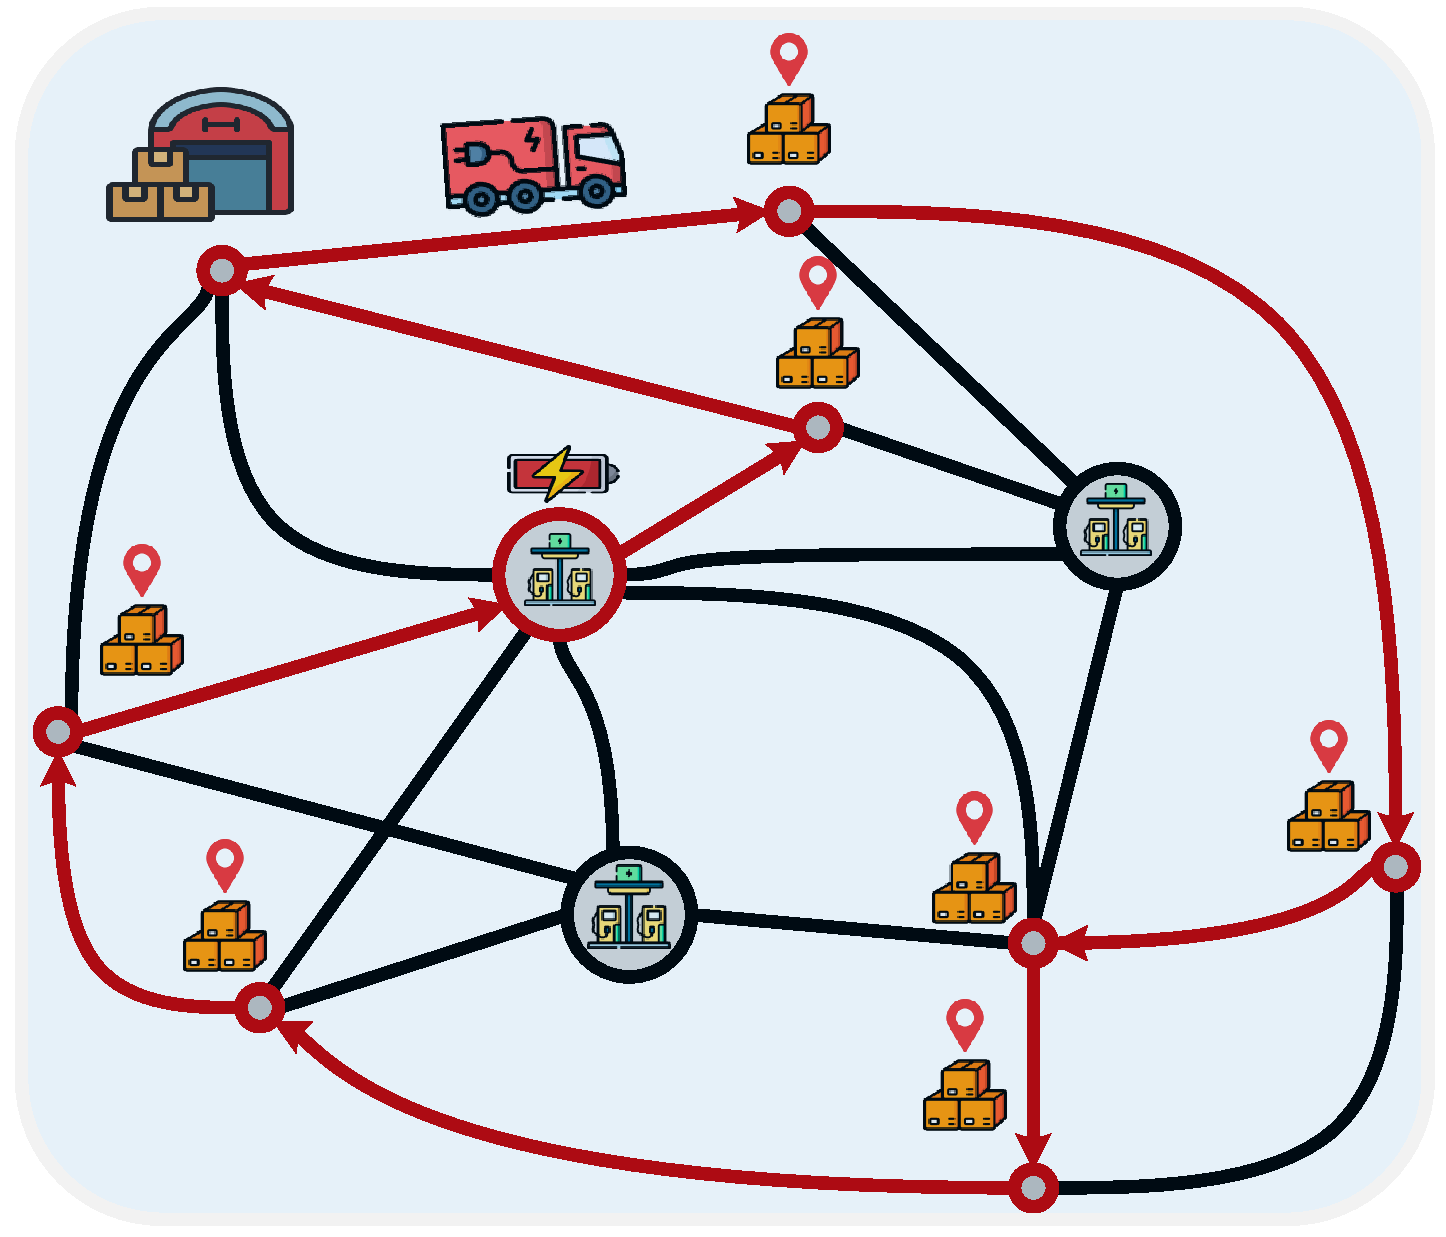
\includegraphics[width=0.4\linewidth]{TruckRoutingProblemOverview_a.pdf}
         \label{fig:ov_a}
         }
     \subfloat[Electric Truck Fleet Routing Problem]{
         \centering
         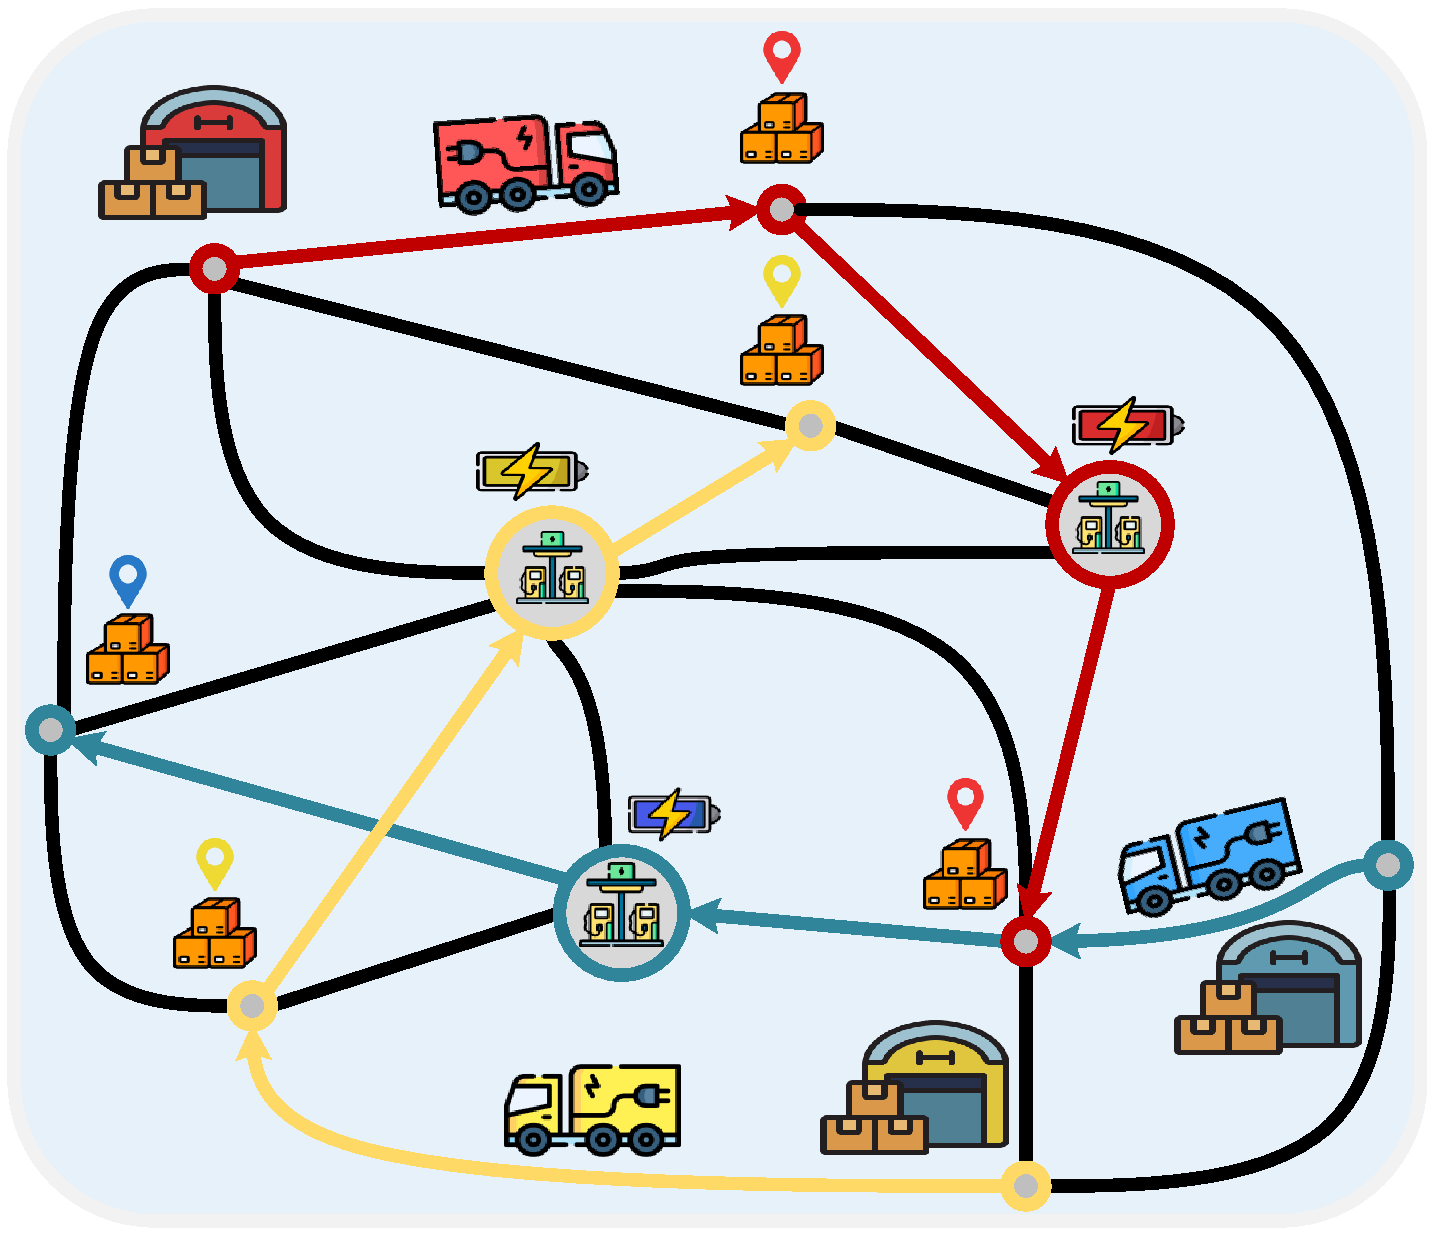
\includegraphics[width=0.4\linewidth]{TruckRoutingProblemOverview_b.pdf}
         \label{fig:ov_b}
         }
        \caption{Comparison of the classic eVRP and the eTFRP with shared charging resources. (a) In eVRP, routing is typically planned for a single vehicle (or independently across vehicles), where charging stops are inserted to maintain energy feasibility along a prescribed tour. (b) In eTFRP, multiple trucks operate concurrently and compete for limited charging capacity, so route execution is coupled through shared stations and potential queuing delays.
        }
        \label{fig:overview}
\end{figure}

The fleet consists of $I$ electric trucks indexed by $\mathcal{I}=\{1,\ldots,I\}$. Each truck $i \in \mathcal{I}$ has battery capacity $\overline{b}_i$ (kWh) and must maintain a minimum energy $\underline{b}_i$ (kWh) to avoid fully discharging and preserve operational safety margins. The initial battery energy of truck $i$ is denoted by $b_i^0$, with the starting value set either to full capacity or sampled from a distribution, depending on the experimental configuration. Each truck starts at a designated depot (or start) node $d_{i}^0\in\mathcal{V}$, which determines the route's initial location. It is possible that every truck starts from a different depot, mirroring the operation of real freight distribution networks~\cite{MOGALE2025111315}.

Delivery points are specified as pre-assigned sets per truck. 
For each truck $i\in\mathcal{I}$, the assigned delivery set is denoted by $\mathcal{D}_i=\{d_{i}^1,\ldots,d_{i}^{K_i}\}$, where $K_i$ is the number of deliveries assigned to truck $i$. In the fixed delivery order mode (sequential), each truck must serve these deliveries in the given order, whereas in the flexible mode (similar to classic eVRP), each truck may choose the order of the remaining deliveries in $\mathcal{D}_i$ to minimize travel time.
Delivery sequences are validated to ensure that each path is feasible under conservative energy assumptions, which may require one or more intermediate charging stops. 

The fixed delivery order in the eTFRP problem differs from that in standard single-vehicle eVRP formulations in two structurally important ways.
First, deliveries are pre-assigned at the truck level (with either sequential or flexible ordering), shifting the operational burden toward energy-feasible execution rather than delivery-to-vehicle assignment. Additionally, in eTFRP, trucks are not necessarily required to return to the initial depot.
Second, charging is a shared resource with finite simultaneous service capacity, so that charging delays depend on the joint behavior of the fleet and cannot be represented as exogenous constants.
Figure~\ref{fig:overview} illustrates this distinction by contrasting the single-vehicle eVRP abstraction with a fleet-level setting in which interactions arise through shared charging infrastructure and associated congestion effects. 

\subsubsection{Sources of Uncertainty}
\label{sec:unc}

Uncertainty enters the problem through exogenous stochasticity in travel times, energy consumption, and unloading durations~\cite{lombard2018modelling}. Travel time on an edge $(u,v)$ departing at time $t$ is modeled as a truncated Gaussian~\cite{RODRIGUES2018636},
\begin{equation}
\tilde{\tau}_{uv}(t) \sim \mathcal{N}\!\big(\tau_{uv},\sigma_{uv}^2(t)\big),
% \qquad
% \tilde{\tau}_{uv}(g)\in[0.85\,\tau_{uv},\,2.5\,\tau_{uv}],
\label{eq:unc_travel}
\end{equation}
where $\sigma_{uv}(t)$ increases during rush-hour periods based on the fraction of the journey interval overlapping rush windows, e.g., in the morning and evening.
Stochastic energy consumption is correlated with traffic to reflect stop-and-go inefficiencies or other truck battery-related nonlinearities, using $\tilde{b}_{uv} = b_{uv}\,\xi_{uv}$. The coefficient $\xi_{uv}$ is defined as:
\begin{equation}
\xi_{uv} =
\operatorname{clip}\!\Big(
1 + 0.5(\tilde{\tau}_{uv}/\tau_{uv}-1) + \varepsilon,\ \underline{\xi},\ \overline{\xi}
\Big),
\label{eq:unc_energy}
\end{equation}
with $\varepsilon\sim\mathcal{N}(0,\sigma_\xi^2)$ representing additional noise, $\sigma_\xi=0.05$. The realized energy is clipped multiplicatively, so that $\tilde{b}_{uv}\in[0.90\,b_{uv},\,1.20\,b_{uv}]$, i.e.\ $\underline{\xi}=0.90$ and $\overline{\xi}=1.20$; the realized travel time is clipped to $\tilde{\tau}_{uv}\in[0.85\,\tau_{uv},\,2.50\,\tau_{uv}]$ and its standard deviation is capped at one hour. Both bounds are applied to the realized quantity and never to the nominal one, so the nominal network $(\tau_{uv},b_{uv})$ that the planners and the feasibility mask read is unaffected by the draw. Throughout, an untilded symbol denotes a nominal quantity and a tilded symbol its realization: $\tau_{uv}$ and $b_{uv}$ are the nominal travel time and energy of edge $(u,v)$, while $\tilde{\tau}_{uv}$ and $\tilde{b}_{uv}$ are the values actually incurred when the edge is traversed. 
Unloading times at delivery nodes can also be stochastic (with realized time $\tilde{q}$), reflecting longer delays during business hours due to facility congestion and dock availability. In this setting, delivery points are assumed to be operational throughout the whole day.

Another source of uncertainty is the endogenous congestion at charging stations. Even if exogenous variables were fixed, the waiting time experienced at a station depends on the arrival times and charging durations of other trucks, making queuing delays a coupled, fleet-level problem. In eTFRP, stations maintain first-come, first-served waitlists and admit trucks to charging ports only when capacity becomes available.

\subsubsection{Objective function and constraints}\label{sec:obj_constraints}

eTFRP is a sequential decision-making problem that requires real-time decisions.
At each decision step $t \in \mathcal{T}$, the operator selects the next action for the active truck, which can be navigating to a delivery location (the next stop in sequential delivery mode or any remaining stop in flexible mode), navigating to a charging station, or, if the truck is currently at a station with access to a charging port, selecting a charging duration $h\in\mathcal{H}$.

Let $\tilde{\tau}^{(i)}_{k}$ denote the realized travel time for the $k$-th travel segment of truck $i$, let $h^{(i)}_{k}$ denote the duration of its $k$-th charging session, let $w^{(i)}_{k}$ denote the waiting time incurred before that charging session due to the congestion at the selected station, and let $\tilde{q}^{(i)}_{k}$ denote the realized unloading time for its $k$-th served delivery. 
The objective is to design a policy $\pi$ that minimizes the expected total time required for the whole fleet to complete all assigned deliveries, formally defined as:
\begin{align}
\min_{\pi}\quad
& \mathbb{E}\!\left[\sum_{i\in\mathcal{I}}
\left(
\sum_{k}\tilde{\tau}^{(i)}_{k}
+
\sum_{k} h^{(i)}_{k}
+
\sum_{k} w^{(i)}_{k}
+
\sum_{k}\tilde{q}^{(i)}_{k}
\right)\right],
\label{eq:obj_time}
\\
\text{s.t.:} \quad
& \underline{b}_i \le b_i(t) \le \overline{b}_i && \forall i\in\mathcal{I}, \ \forall t \in \mathcal{T},
\label{eq:con_battery_bounds}
\\
& \alpha\cdot e_{n_i(t),v} < b_i(t) && \forall i\in\mathcal{I},\ \forall t \in \mathcal{T},
| \; i\mapsto \text{navigates}(v),
\label{eq:con_energy_headroom}
\\
& b_i\!\left(t+\tilde{\tau}_{n_i(t),v}\right)= b_i(t)-\tilde{e}_{n_i(t),v} && \forall i\in\mathcal{I},\ \forall t \in \mathcal{T}\ | \; i\mapsto \text{navigates}(v),
\label{eq:con_energy_update_travel}
\\
& b_i(t+h)=\min\!\Big\{\overline{b}_i,\ b_i(t)+ \int_{0}^{h}\eta_c \, P_c\!\left(\mathrm{soc}_i(t+s)\right)\, ds \Big\}, \quad \frac{\mathrm{d}\,\mathrm{soc}_i(t+s)}{\mathrm{d}s} = \frac{\eta_c\,P_c(\mathrm{soc}_i(t+s))}{\overline{b}_i} && \forall i\in\mathcal{I},\ \forall t \in \mathcal{T}\ | \; i\mapsto \text{charges}(c,h),
\label{eq:con_energy_update_charge}
\\
& |\mathcal{M}_c(t)| \le \kappa_c && \forall c\in\mathcal{C}, \ \forall t \in \mathcal{T}.
\label{eq:con_ports}
\end{align}

In Eq.~\eqref{eq:con_energy_update_charge} the integration variable $s$ is the elapsed charging time, distinct from the wall-clock time $t$ at which the session begins, and the integrand is evaluated along the \emph{state-of-charge trajectory} $\mathrm{soc}_i(t+s)$ rather than at the fixed initial state $b_i(t)$. This distinction is not cosmetic: because the power curve $P_c(\cdot)$ tapers above a threshold state of charge, holding the argument at its initial value would overstate the energy delivered by a session that crosses the taper, and by up to $55\%$ for a session ending near a full battery. The simulator integrates the same trajectory numerically, and the feasibility mask, the heuristic, and both planners price a recharge with that identical routine, so no method plans against a charging model the simulator will not execute.
Here $b_i(t)$ denotes the battery energy of truck $i$ at time $t$, $n_i(t)\in\mathcal{V}$ denotes its current location node, and $\mathcal{M}_c(t)\subseteq\mathcal{I}$ denotes the set of trucks occupying charging ports at station $c$ at time $t$. 
Constraints~\eqref{eq:con_battery_bounds} and \eqref{eq:con_energy_headroom} enforce energy feasibility throughout the operational day. The battery bound in~\eqref{eq:con_battery_bounds} maintains a minimum buffer $\underline b_i$ and prevents exceeding capacity $\overline{b}_i$. In detail, constraint~\eqref{eq:con_energy_headroom} requires that any selected navigation action to a node $u$ is feasible under a safety multiplier $\alpha\ge 1$, which conservatively accounts for energy uncertainty. 
The battery evolution is captured explicitly by~\eqref{eq:con_energy_update_travel} and \eqref{eq:con_energy_update_charge}.
In~\eqref{eq:con_energy_update_travel}, $\tilde{e}_{uv}$ and $\tilde{\tau}_{uv}$ denote the realized energy consumption and travel time on edge $(u,v)$. In~\eqref{eq:con_energy_update_charge}, the function $P_c(\cdot)$ returns the energy added over duration $h$ at station $c$ given charging efficiency $\eta_c$ and the station-specific max charging power $\overline{p}_c$. Its explicit charging curve equation is specified in Section~\ref{sec:charging_model}.

Constraint~\eqref{eq:con_ports} captures the coupling introduced by shared charging resources. In particular, \eqref{eq:con_ports} limits the number of trucks that can charge simultaneously at station $c$ and induces a first-come, first-served waiting time $w_k^{(i)}$ when a truck arrives while all $\kappa_c$ ports are occupied. 
By doing that, the realized waiting terms $\{w_k^{(i)}\}$ in~\eqref{eq:obj_time} are determined by the interaction of simultaneous routing and charging decisions across the fleet.


\subsection{Event-driven Simulation Environment}\label{sec:sim_env}

To enable reproducible evaluation of different eTFRP solutions, the mathematical problem is transformed into an event-driven simulation environment that executes fleet operations in continuous time. 
The simulator maintains a priority queue of timestamped events ($t\in \mathcal{T}$), and advances time by repeatedly processing the earliest event in the queue. This design avoids fixed-step discretization artifacts and naturally supports heterogeneous action durations, including travel segments of different lengths, charging sessions of variable duration, and unloading times.
At each event, the simulator updates the system state (truck locations, battery levels, station occupancies, and queues) and schedules subsequent events induced by the executed action, such as arrival at the next node, completion of charging, or completion of unloading.
The simulator environment uses the Gymnasium API~\cite{brockman2016openai} and is suitable for the development and testing of RL algorithms while also supporting mathematical programming and heuristic planning algorithms.

\begin{figure}
    \centering
    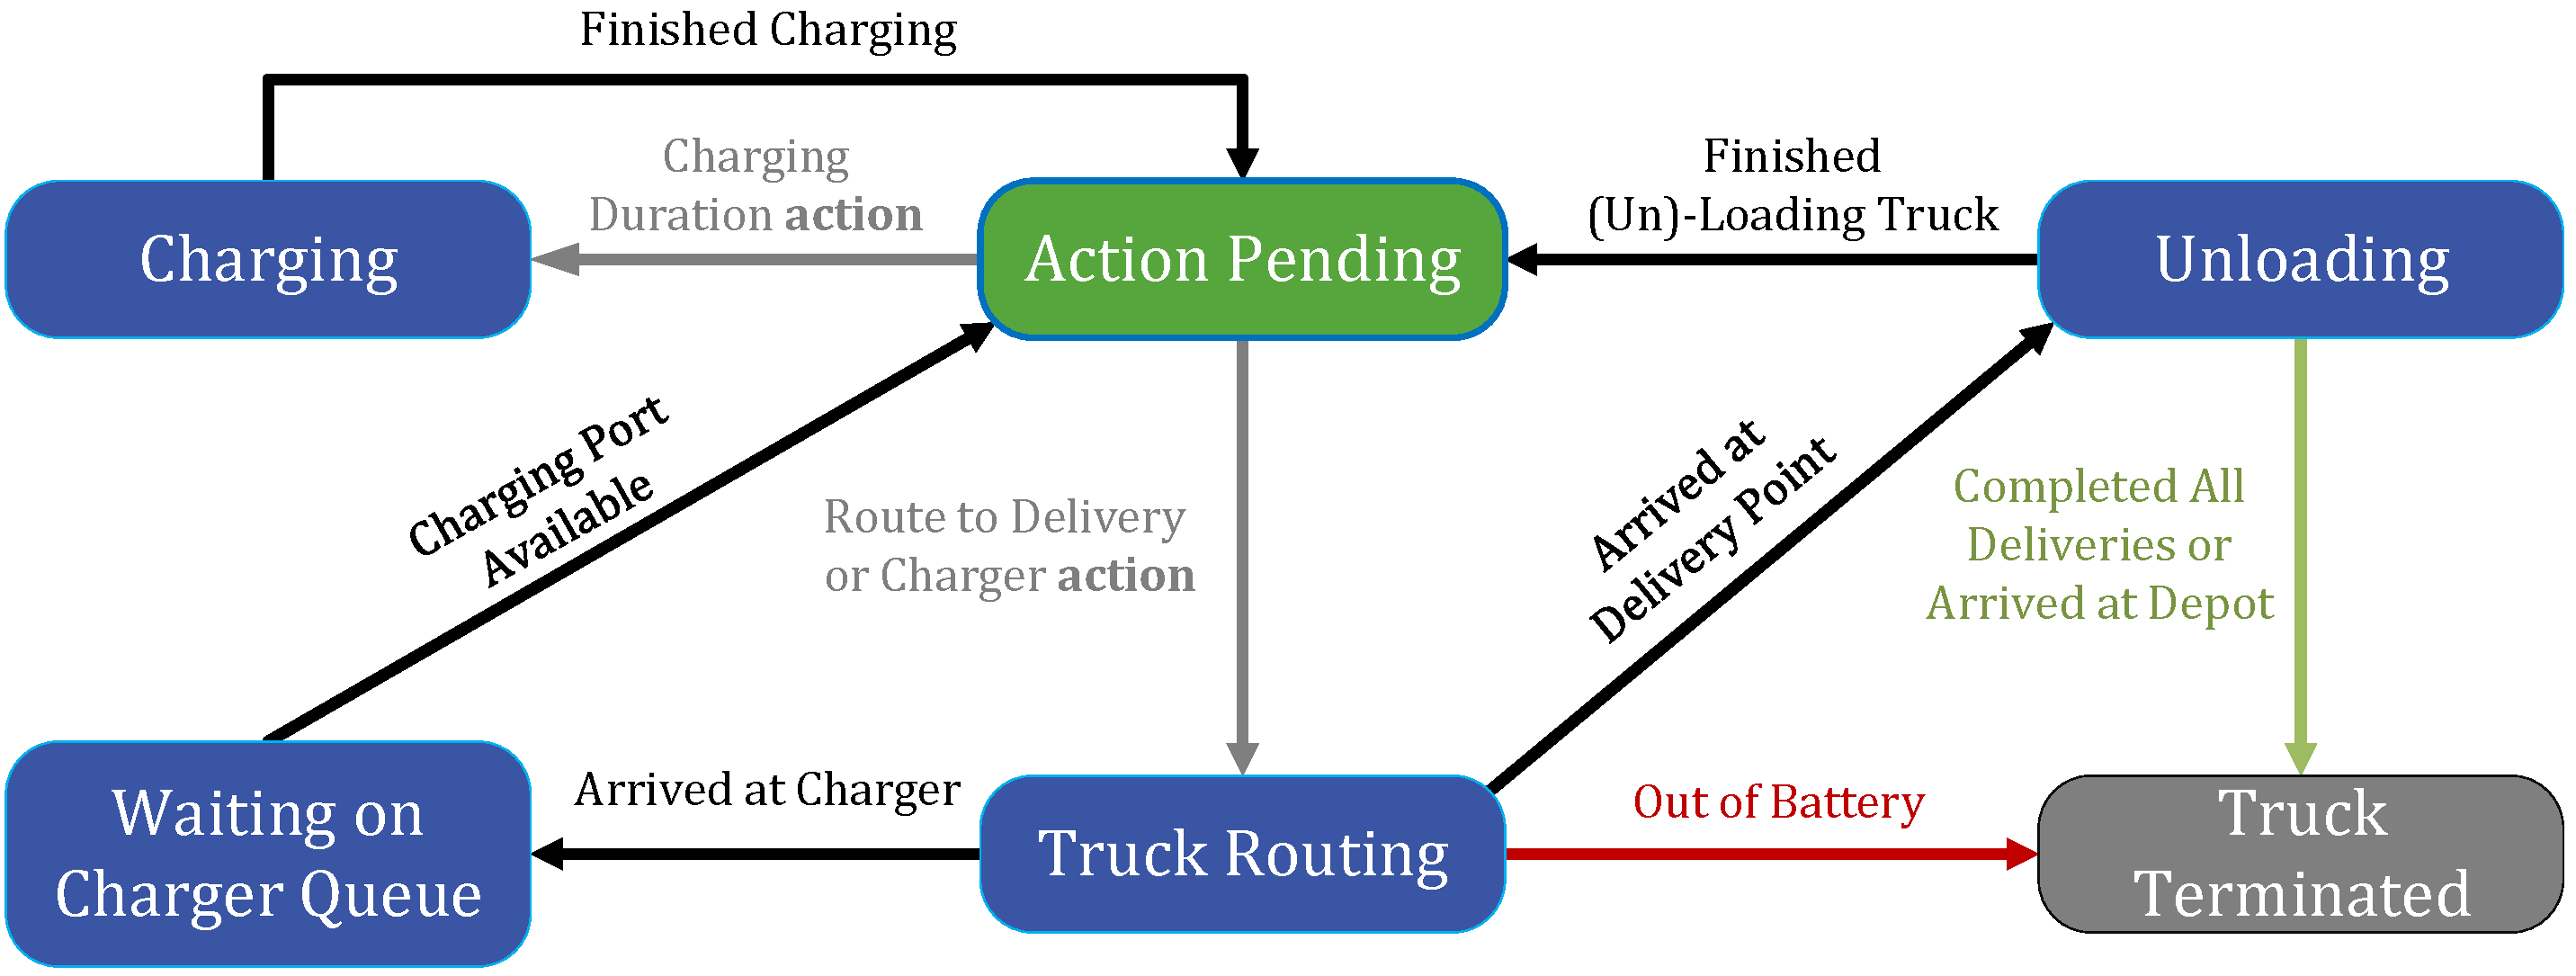
\includegraphics[width=0.8\linewidth]{TruckStateMachine_cropped.pdf}
    \caption{Event-driven truck state machine used by the simulator. Decision steps occur when a truck becomes \texttt{ready}; arrivals, charging, unloading, and FCFS (first-come, first-served) queuing trigger subsequent events.}
    \label{fig:truck_state_machine}
\end{figure}

Each truck transitions among a finite set of operational states that define when it can accept a new decision and when it is constrained by ongoing activities.
In particular, a truck may be in the states: \texttt{Action\_Pending} (available to act), \texttt{Routing} (travel in progress), \texttt{Waiting\_on\_Charger\_Queue} (queued at a station), \texttt{Charging} (occupying a port), \texttt{Unloading} (service in progress), or \texttt{Terminated}, when all deliveries are complete or the truck is out of battery. 
A decision must be made whenever a truck enters the \texttt{Action Pending} state, which occurs after completing a travel segment, finishing unloading at a delivery, or finishing (and vacating) a charging port. 
The resulting event-driven decision structure for each truck is summarized by the state machine in Figure~\ref{fig:truck_state_machine}.

\subsubsection{Charging model}\label{sec:charging_model}
The simulator implements a realistic battery charging model that better reflects DC fast charging than the linear models commonly used in the literature (e.g.,~\cite{BASSO2022102496,lin2022,11016767}).  
During charging, the battery energy increases according to Equation \eqref{eq:con_energy_update_charge}.
In detail, the function $P_c(\cdot)$ returns the net energy added over $[t,t+h]$ and, for DC fast charging, is designed to capture Constant Current--Constant Voltage (CCCV) dynamics through a state of charge (SoC)-dependent tapered power profile. Let $\overline{p}_c$ and $\underline{p}_c$ denote the station-specific peak and minimum charging powers, with SoC defined as $b/\overline{b}$ taking values in $[0,1]$. 
The CCCV charging power is inspired by~\cite{10225616}, and is modeled as a piecewise function:
\begin{equation}
P_c(\text{SoC})=
\begin{cases}
\overline{p}_c \cdot (0.6+3.0 \cdot \text{SoC}), & \text{SoC}\in[0,0.10],\\
\overline{p}_c \cdot\big(0.9+0.25\,(\text{SoC}-0.10)\big), & \text{SoC}\in(0.10,0.50],\\
\overline{p}_c, & \text{SoC}\in(0.50,0.80],\\
\max\!\Big(\underline{p}_{c},\;\overline{p}_c\big(1-0.6\,p^{1.5}\big)\Big), & \text{SoC}\in(0.80,1.0],\;\; \text{where}\,\, p=\frac{\text{SoC}-0.80}{0.20},
\end{cases}
\label{eq:cccv_profile}
\end{equation}
which produces a near-constant-power region at mid SoC and a taper at high SoC. 
% Given the battery energy $b$ at time $t$, and a SoC trajectory SoC during charging, the net energy added over a charging duration $h$ is defined as follows:
% \begin{equation}
% f\!\big(\eta_c,\overline{p}_c,b_i(t),h\big)
% =\int_{t}^{t+h}\eta_c \cdot p_c\!\left(\frac{b_i(t)}{\overline{b}_i}\right)\, dt,
% \label{eq:f_cccv_oneline}
% \end{equation}
In the simulator, \eqref{eq:con_energy_update_charge} is implemented as a discrete integration with a small step $dt$, iteratively updating $b(t)$ and the corresponding SoC-dependent power over $[t,t+h]$. %Notice that unlike the classi~\cite{10225616}

\begin{figure}
    \centering
    
\includegraphics[width=0.75\linewidth]{charging_curve_comparison.pdf}
    \caption{Charging power profile and SoC evolution under constant-power (linear) charging versus tapered CCCV fast charging. Tapering reduces effective power at high SoC and changes optimal charging durations.}
    \label{fig:charging_curve}
\end{figure}

The aforementioned charging model is important for electric truck operations because DC fast charging does not maintain constant power over the full SoC range. Instead, charging power typically tapers as SoC approaches high values, producing diminishing returns in energy gained per unit time. Figure~\ref{fig:charging_curve} visualizes the contrast between a linear charging model and a tapered fast-charging curve, highlighting why decisions about how long to charge cannot be approximated reliably by a linear model at high SoC.





% \newpage


%%%% ==========================================================================================
%%%% ==========================================================================================
%%%% ==========================================================================================
\section{Learning-Based Electric Truck Fleet Routing}

In this section, the eTFRP is formulated as an event-driven semi-Markov Decision Process (SMDP) with a heterogeneous graph state representation and a feasibility-aware, variable-size action representation that mirrors the operational constraints of the truck routing problem. 
Building on this formulation, a graph-based actor-critic architecture and a variable-action GraphPPO training procedure are introduced to enable scalable and generalizable decision-making across instances with varying fleet sizes, delivery sets, and charging infrastructure.



\begin{figure}
    \centering
    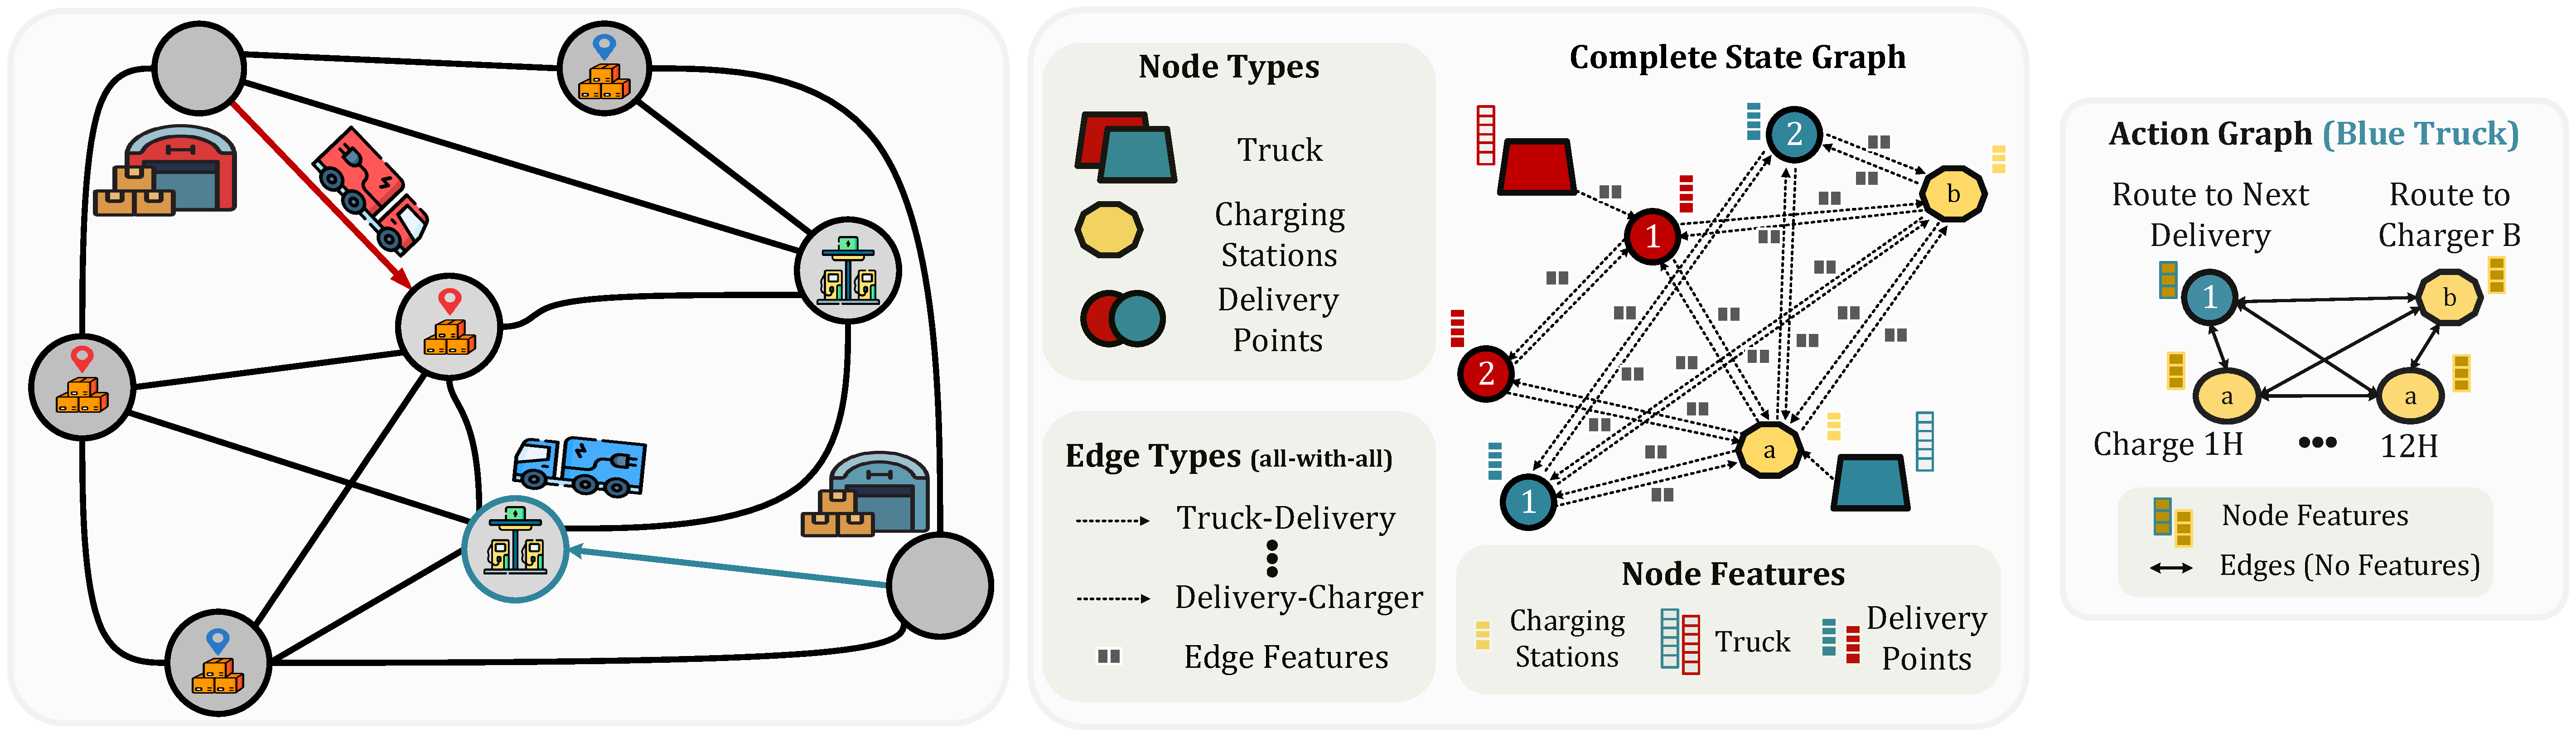
\includegraphics[width=0.98\linewidth]{TruckGraph.pdf}
    % \caption{Illustration of the process of turning the problem state at a step to a state and action graph, by converting objects to distinct nodes, e.g., trucks, chargers, deliveries.}
    \caption{Illustration of the graph construction process at a decision step. The current system state is transformed into a heterogeneous state graph by representing trucks, charging stations, and delivery locations as distinct node types, while feasible routing and charging decisions are encoded in a corresponding action graph.}
    \label{fig:graph_conv}
\end{figure}




\subsection{Graph-Based Semi Markov Decision Process}\label{sec:smdp}
The eTFRP operates in continuous time, and decisions are requested only when a truck enters the \texttt{Action\_Pending} state. 
This event-driven nature of the problem, where each decision step doesn't consist of fixed time intervals, leads to an SMDP~\cite{Elsevier2013_ISBN9780124077959} defined by the tuple
$\big(\mathcal{S},\{\mathcal{A}(s)\}_{s\in\mathcal{S}},P,r,\gamma\big)$,
where $s_t\in\mathcal{S}$ denotes the state observed at the $t$-th decision step, $\mathcal{A}(s_t)$ is the state dependent action space, $P$ is a transition kernel that governs both the next state and the holding time between decisions, $r$ is the reward, and $\gamma\in(0,1)$ is a discount factor. 
% Let $\{g_t\}_{t\ge 0}$ denote the increasing sequence of global times at which decision epochs occur (i.e., \textsc{TRUCK\_READY} events in the event-driven simulator), and define the random holding time $\Delta t_t \triangleq g_{t+1}-g_t$.
The SMDP transition kernel is denoted $P(s_{t+1} \mid s_t, a_t)$ and is determined by the event-driven dynamics introduced in Equations~\eqref{eq:con_battery_bounds}-\eqref{eq:con_ports}. After taking action $a_t$ at state $s_t$, the simulator advances time until the next event (e.g., when a truck is in the ``Action Pending" state) and returns the corresponding next state $s_{t+1}$. 

\subsubsection{The state space}

At each decision step $t$, only a single truck becomes active. If multiple trucks are ready at the exact same time, one is randomly selected; this is rare. 
The state $s_t$ not only contains the state of the active truck $i$, but also contains the full system state needed to evaluate feasibility and to simulate subsequent evolution. The state $s_t\in \mathcal{S}$ is represented as a heterogeneous graph $\mathcal{G}^{\mathcal{S}}_t(\mathcal{V}^{\mathcal{S}}_t,\mathcal{E}^{\mathcal{S}}_t) \subset \mathcal{G}(\mathcal{V},\mathcal{E})$ built on the same entities and symbols used in the problem formulation described in Section~\ref{sec:problem_definition}.
Specifically, as illustrated in Figure~\ref{fig:graph_conv}, a snapshot of the whole eTFRP system state can be converted into the state graph $\mathcal{G}^{\mathcal{S}}_t$ containing three node types comprising the node set $\mathcal{V}^{\mathcal{S}}_t$. Truck nodes are indexed by $i\in\mathcal{I}$, delivery nodes indexed by $d\in\mathcal{D}$, and charging-station nodes indexed by $c\in\mathcal{C}$.

Each truck node has a feature vector $x^{\mathrm{Truck}}_i(t)\in\mathbb{R}$ defined as
\begin{equation}
x^{\mathrm{Truck}}_i(t)\;=\;
\Big[
\frac{b_i(t)}{\overline{b}_i},\;
% i,\;
\text{status}_i(t),\;
% \frac{k_i^{\text{done}}(t)}{K_i},\;
\frac{|\mathcal{D}^*_i(t)|}{K_i},\;\
\frac{t_i^{\text{elapsed}}(t)}{T},\;
% \frac{\tau_i^{\text{traveled}}(t)}{1000},\;
\frac{t_i^{\text{arrival}}(t)}{T}
\Big]^\top,
\;\;\;\quad \forall i \in \mathcal{I},
\label{eq:truck_features}
\end{equation}
where the first term is the SoC of the truck, the second term denotes the operational status of truck $i$ in the event-driven simulator with a normalized one-hot encoding (e.g., \texttt{ready}, \texttt{routing}, \texttt{charging}, \texttt{waiting\_to\_charge}, \texttt{unloading}).
The set $|\mathcal{D}^*_i(t)| \in \{1,\dots, {K_i}\}$ denotes the number of remaining deliveries for truck $i$, while $K_i$ is the total number of deliveries; hence, the third term is the normalized number of remaining deliveries. The scalar $t_i^{\text{elapsed}}(t)$ denotes the elapsed time since the start of truck $i$'s episode (normalized by the maximum simulation time $T$).
% and $d_i^{\text{traveled}}(t)$ denotes the cumulative distance traveled.
Finally, $t_i^{\text{arrival}}(t)$ shows the estimation of the next ``Action Pending'' event of truck $i$, so it would be zero for the active truck. 

Each pending delivery node for truck $i$ at step $t$ ($d\in\mathcal{D}^*_i(t) \subseteq \mathcal{D}_i$) is associated with feature vector
\begin{equation}
x^{\mathrm{Delivery}}_d(t)\;=\;
\Big[
d_{i,k},\;
|\mathcal{D}^{*}_{i}(t)|,\;
\Big]^\top,
\;\;\;\quad \forall i \in \mathcal{I}, \; \forall d_i \in \mathcal{D}_{i}^*(t).
\label{eq:delivery_features}
\end{equation}
Note that already completed deliveries no longer need to be included in the state space as nodes, as they no longer affect future decisions.

Finally, each charging-station node $c\in\mathcal{C}$ has a feature vector defined as:
\begin{equation}
x^{\mathrm{Charger}}_c(t)\;=\;
\Big[
c,
\overline{p}_c,\;
\eta_c,\;
\kappa_c,\;
\frac{|\mathcal{M}_c(t)|}{\kappa_c},\;
q_c(t)
\Big]^\top,
\forall c \in \mathcal{C}
\label{eq:charger_features}
\end{equation}
where $\overline{p}_c$ is the station peak power, $\eta_c$ the charging efficiency, $\kappa_c$ the number of charging ports, $\mathcal{M}_c(t)\subseteq\mathcal{I}$ the set of trucks occupying ports at time $t$ (as in~\eqref{eq:con_ports}), and $q_c(t)$ denotes the charger queue length at station $c$ at time $t$. Charging prices are assumed to be homogeneous across the traffic network; therefore, they are excluded from the charger state vector.

The edges $\mathcal{E}_t$ of the graph are designed to reflect the transportation costs between all available nodes, as shown in the state graph of Figure~\ref{fig:graph_conv}.
Edges are constructed for each pair of nodes $v,u\in\mathcal{C}\cup\mathcal{D}^*(t)\cup\mathcal{I}$, each with features:
\begin{equation}
x^{\mathrm{Edge}}_{uv}(t)\;=\;\big[\tau_{uv},\; e_{uv}\big]^\top.
\label{eq:edge_features}
\end{equation}
% using the base travel time $\tau_{uv}$ and base energy requirement $e_{uv}$ defined on the directed graph $G=(\mathcal{V},\mathcal{E})$. 
Since $\mathcal{G}$ is not assumed symmetric, these edge features generally satisfy $x^{\mathrm{edge}}_{uv}(t)\neq x^{\mathrm{edge}}_{vu}(t)$ when reversing direction, capturing direction-dependent travel and energy costs.

\subsubsection{The feasible action space}\label{sec:feasible_actions}

The action space in eTFRP is state-dependent because at each decision step only a subset of routing and charging decisions is feasible given the active truck's location, its available battery energy, the set of remaining deliveries, and the instantaneous availability of charging ports. 

To reduce the number of available action combinations, actions that navigate trucks to chargers are limited using a detour-based screening heuristic. 
Let $\bar{d}_{i}(t)$ denote a reference delivery used to measure detours, defined as $\bar{d}_{i}(t)=d_{i}^{k_{i}(t)+1}$ in sequential mode and as the closest remaining delivery in flexible mode.
For each charging station $c\in\mathcal{C}$, the incremental detour (in nominal travel time) of visiting $c$ before continuing toward $\bar{d}_{i_t}(t)$ is computed as
\begin{equation}
\Delta \tau _{i,c} \;=\;\tau_{n_{i}(t),c}+\tau_{c,\bar{d}_{i}(t)}-\tau_{n_{i}(t),\bar{d}_{i}(t)}.
\label{eq:charger_detour}
\end{equation}
Only the $k^{\mathrm{chg}}$ chargers with the smallest detour durations are retained as candidates.
The resulting set of candidate navigation destinations is then
$\hat{\mathcal{V}}_{t}:\{\mathcal{C}^{K_{\mathrm{chg}}}_{i}(t)\ \cup\ \mathcal{D}^{*}_{i}(t)$\}.
This screening step focuses decisions on chargers that are nearby in terms of incremental route deviation, which is particularly relevant in freight operations, where large detours are unlikely to be attractive unless necessitated by feasibility constraints.
Furthermore, a navigation decision to $v\in\hat{\mathcal{V}}_{t}$ is feasible only if it satisfies the conservative energy condition introduced in~\eqref{eq:con_energy_headroom}. This yields the feasible navigation action set
\begin{equation}
\mathcal{A}^{\mathrm{nav}}(s_t)\;=\;\Big\{\;\text{navigate}(v)\;:\; v\in \hat{\mathcal{V}}_{t},\ \alpha\,e_{n_{i}(t),v}<b_{i}(t)\;\Big\},
\label{eq:feasible_nav}
\end{equation}
which filters candidate destinations by requiring sufficient battery energy under the safety multiplier $\alpha\ge 1$.

Charging decisions are only meaningful when the active truck is at a charging station and can initiate charging.
$\mathcal{M}_c(t)\subseteq\mathcal{I}$ is the set of trucks occupying ports at station $c$ at time $t$, and recall that at most $\kappa_c$ trucks can charge simultaneously.
When $n_i(t)=c\in\mathcal{C}$ and a port is available, the truck may select a charging duration $h$ from a discrete set $\mathcal{H}$, which is used to model operationally realistic charging decisions at coarse time intervals. In this work, $\mathcal{H}=\{1,2,\ldots,12\}$ (hours), since a truck should not require more than 12 hours to fully charge, considering fast chargers. The feasible charging actions are therefore
\begin{equation}
\mathcal{A}^{\mathrm{chg}}(s_t)\;=\;\Big\{\;\text{charge}(c,h)\;:\; c=n_{i}(t)\in\mathcal{C},\ |\mathcal{M}_c(t)|<\kappa_c,\ h\in\mathcal{H}\;\Big\}.
\label{eq:feasible_charge}
\end{equation}
The overall feasible action set at step $t$ is given by
$\mathcal{A}(s_t)\;=\;\mathcal{A}^{\mathrm{nav}}(s_t)\ \cup\ \mathcal{A}^{\mathrm{chg}}(s_t)$,
and can equivalently be represented through a binary feasibility mask $m(s_t)$.

The cardinality of $\mathcal{A}(s_t)$ varies across decision steps because both $\mathcal{D}^{*}_{i}(t)$ and the feasibility condition in~\eqref{eq:feasible_nav} depend on the active truck's state, and because charging actions are available only when $n_i(t)\in\mathcal{C}$ and station capacity remains.
For algorithms that require a fixed action dimension (i.e., most RL implementations), a natural upper bound is obtained by enumerating all destination-based navigation actions and all charging-duration actions, yielding a fixed action set size of
$ \lceil\mathcal{A}\rceil \;=\;|\mathcal{C}| \;+\; |\mathcal{D}_{i}(t)| \;+\; |\mathcal{H}|$,
with infeasible actions suppressed at runtime via the binary mask $m(s_t)$.

As shown in Figure~\ref{fig:graph_conv}, at each step $t$, the action set $\mathcal{A}(s_t)$ is also encoded as an action graph $\mathcal{G}^{\mathcal{A}}_t=(\mathcal{V}^{\mathcal{A}}_t,\mathcal{E}^{\mathcal{A}}_t)$,
where $\mathcal{V}^{\mathcal{A}}_t$ contains one node per feasible action. The graph is fully connected with no edge features since the edges do not have a physical meaning, unlike the state graph, where edges represent physical trip distances. 
Each action node $a$ has a three-dimensional feature vector
\begin{equation}
x^{\text{Action}}(t)=\big[\ \mathrm{type}(a),\ \widehat{b}(a),\ \widehat{t}(a)\ \big]^\top,
\label{eq:action_node_features}
\end{equation}
where $\mathrm{type}(a)$ identifies the action category (navigate-to-delivery, navigate-to-charger, or charge),
$\widehat{b}(a)$ is the estimated battery energy after executing $a$ using the nominal updates in \eqref{eq:con_energy_update_travel}--\eqref{eq:con_energy_update_charge}, and
$\widehat{t}(a)$ is the estimated completion time based on the nominal duration of the routing or charging action. 
A graph-based representation of the state and the feasible action set enables GNN policies to exploit network structure while restricting decisions to feasible actions, thereby improving sample efficiency and generalization across varying fleet and infrastructure sizes.

\subsubsection{Reward function}\label{sec:reward}
A time-based reward is adopted to align the learning with the eTFRP objective function in~\eqref{eq:obj_time}, while providing additional shaping signals that encourage task completion and discourage unsafe behavior.
The reward is defined as:
\begin{equation}
r(s_t,a_t,s_{t+1})
=
-\lambda_1\,\Delta t_i
+\lambda_2\,\{\text{delivery completed at }t\}
+\;\lambda_3\,\{\text{failure at }t\},
% -\lambda_1\,\Delta t^{\mathrm{wait}}_i,
\label{eq:reward}
\end{equation}
where $\Delta t_i$ is the time passed since the last ``action pending'' status of truck $i$, comprising the realized travel duration on the selected road-network transition, the realized unloading time, the charging duration, and any waiting incurred in a charger queue.
This choice ensures that the reward directly reflects the operational time consumed by routing, service, and charging decisions under uncertainty. 
Furthermore, $\lambda_1>0$ and $\lambda_2>0$ are scalar coefficients, and $\lambda_3<0$ is a terminal penalty.
The delivery completion term $\lambda_2$ provides a sparse positive signal whenever a truck successfully completes a delivery, improving exploration and encouraging policies that complete assigned tasks efficiently.
% In practice, delivery completion is detected when a truck arrives at a non-depot delivery location and finishes the corresponding unloading process, at which point the indicator $\mathbb{I}\{\text{delivery completed at }t\}$ is set to one.
The failure term $\lambda_3$ is applied when the battery is depleted during a routing segment or when the truck becomes stranded without a feasible continuation. The terminal penalty is set to a sufficiently large magnitude to discourage risky decisions that violate energy feasibility, complementing the conservative feasibility logic used in the action set construction.

\subsection{Graph Actor-Critic Network Architecture}\label{sec:gnn_arch}

\begin{figure}
    \centering
    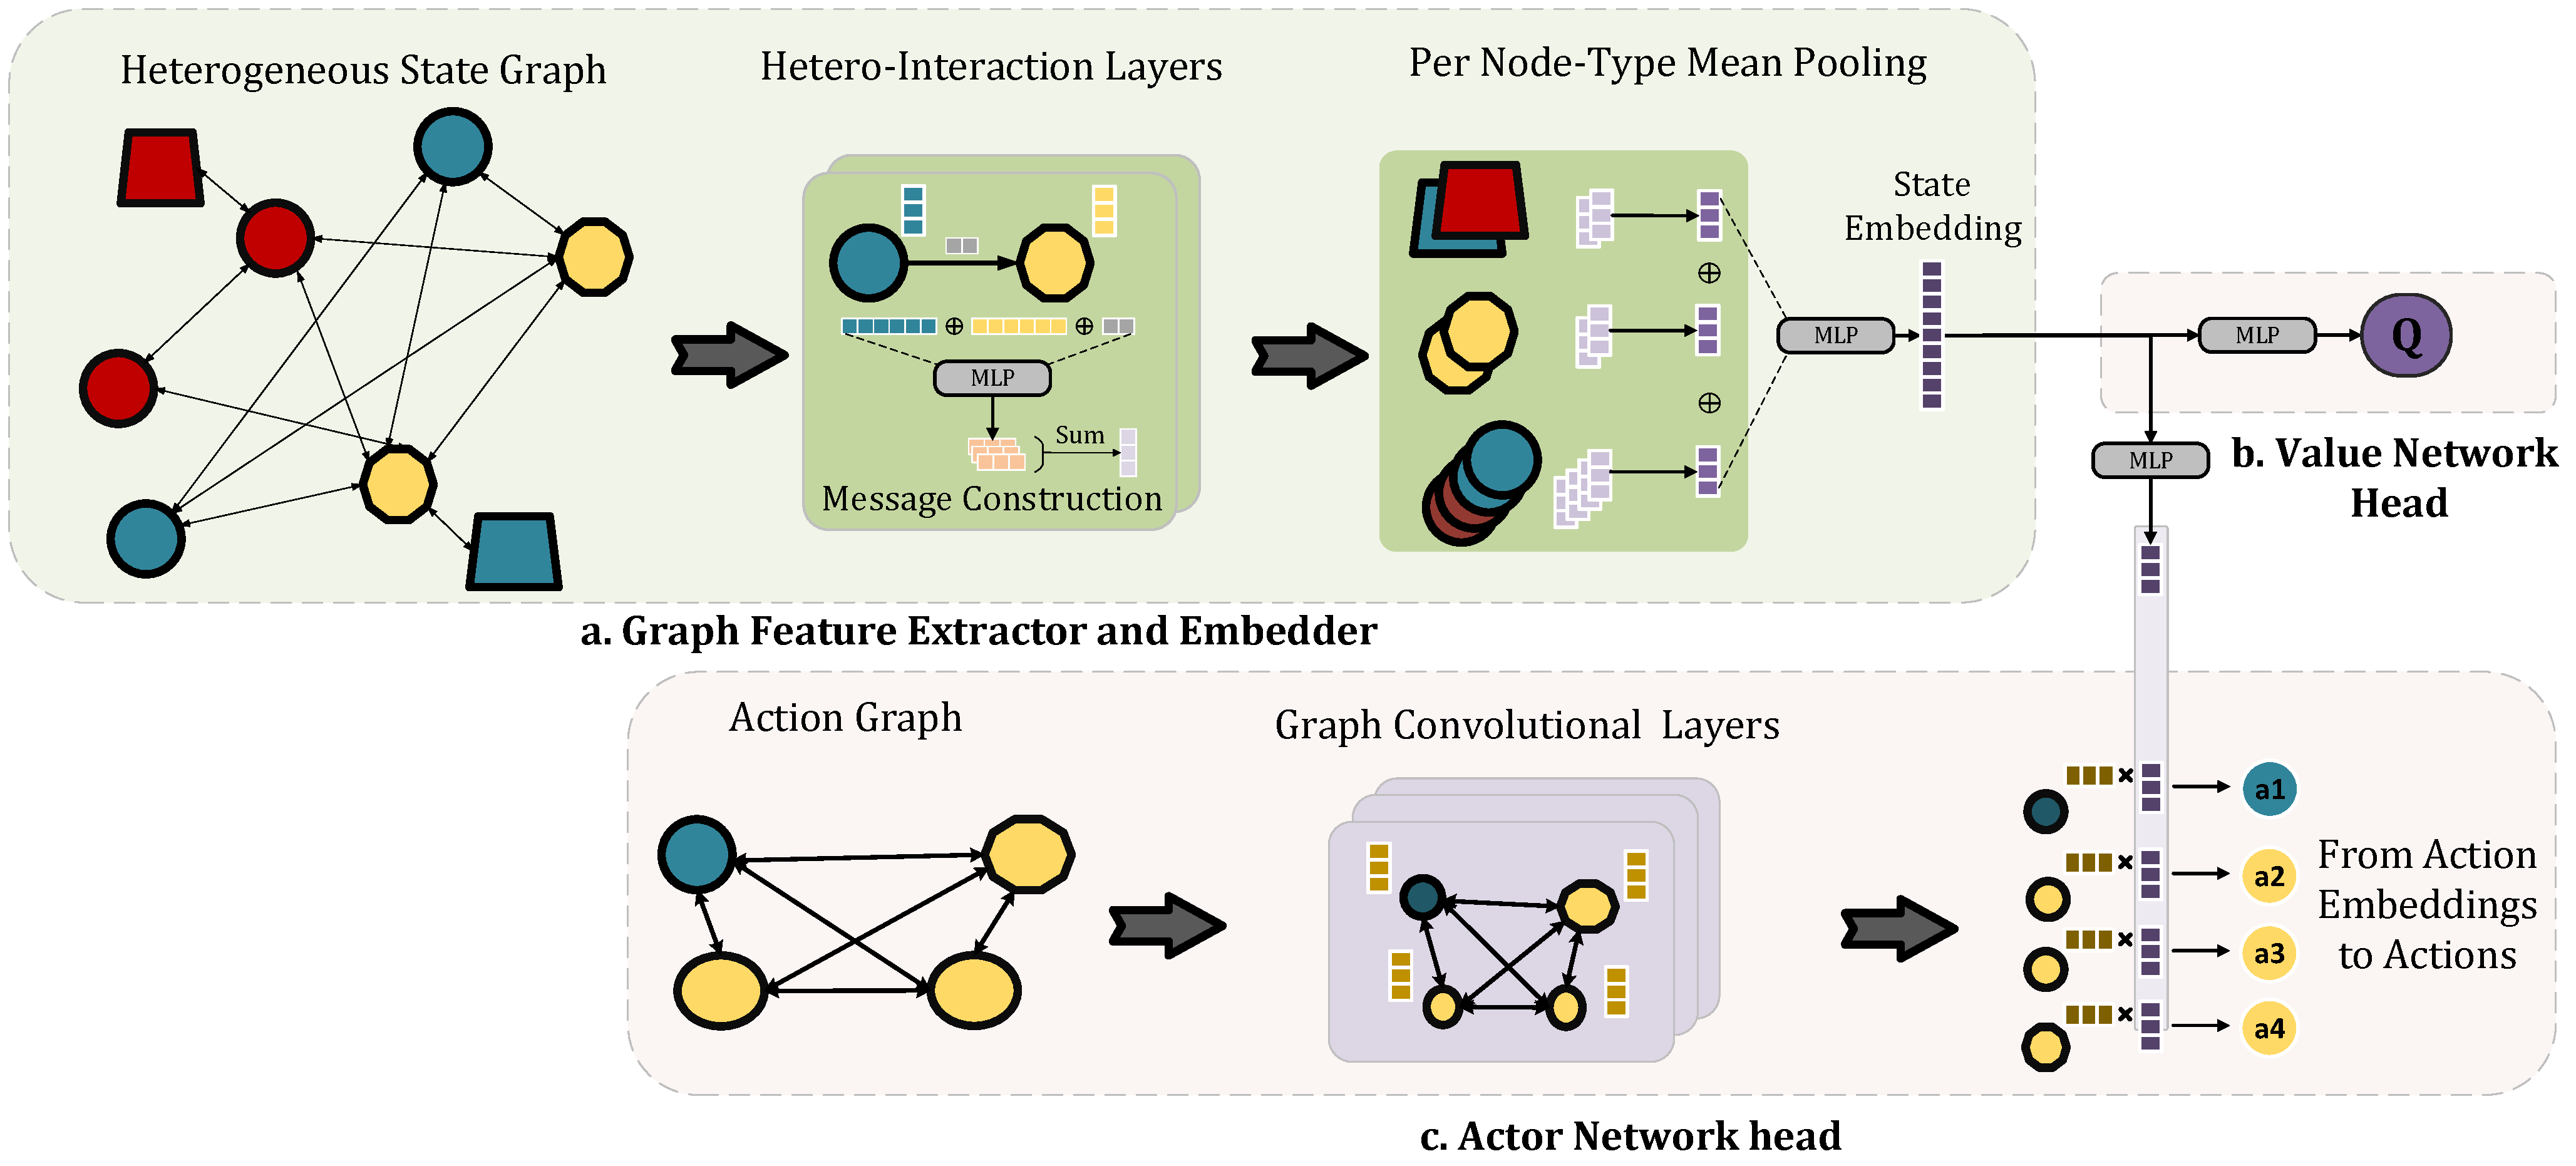
\includegraphics[width=0.8\linewidth]{TruckNetwork.pdf}
    % \caption{The proposed actor-critic neural network that can process the state and action graphs to generate actions and value estimation. }
    \caption{Proposed graph-based actor--critic architecture. In (a), the heterogeneous state graph is encoded through graph feature extraction, hetero-interaction layers~\cite{arowolo2025generalizationgraphneuralnetworks}, and per-node-type mean pooling to obtain a fixed-size global state embedding, invariant to the number of nodes in the state. In (b), the critic head maps this state embedding to a state-value estimate. In (c), the actor head processes the feasible-action graph through graph convolutional layers and combines the resulting action embeddings with the state embedding to produce a policy over routing and charging actions.}
    Panels are referred to throughout as (a) State Graph Encoder, (b) Action Graph Encoder, and (c) Actor Network Head; the panel captions inside the figure asset use the same names.
    \label{fig:graph}
\end{figure}


Representing both the system state and the feasible action set as graphs enables an actor--critic architecture that exploits the relational structure of the transportation network and the shared charging infrastructure, while remaining invariant to the number of trucks, deliveries, and charging stations.
The proposed actor and critic networks, visualized in Figure~\ref{fig:graph}, consist of a shared heterogeneous graph encoder that maps the state graph $\mathcal{G}^{\mathcal{S}}_t$ to latent representations, followed by (i) an actor head that scores the nodes of the action graph $\mathcal{G}_t^{\mathcal{A}}$ and creates a categorical policy over $\mathcal{A}(s_t)$, and (ii) a critic head that estimates the state value from a state embedding representation of $\mathcal{G}^{\mathcal{S}}_t$.

\subsubsection{State Graph Encoder}

Initially, the heterogeneous state graph $\mathcal{G}^{\mathcal{S}}_t$ is passed through node specific encoders $f_j(x^j)$ producing node embeddings $\{h_j^{(l)}\}$ for each layer $l$ where $j\in\{\mathrm{Truck},\mathrm{Delivery},\mathrm{Charger}\}$ denotes the node type (as defined in Section~\ref{sec:smdp}).
Each node encoder starts with a single-layer Multilayer Perceptron (MLP), defined as $h_j^{(l)}(x)=W^{(l)}_{j}x+b^{(l)}_{j}$ with the trainable matrix $W^{(l)}\in\mathbf{R}^{F_{l-1} \times F_{l}}$ and bias vector $b^{(l)}\in\mathbf{R}^{F_{l}}$, where $F_{l}$ is the number of hidden nodes.
The node embeddings are then refined through $L$ graph \emph{Hetero-Interaction} layers~\cite{arowolo2025generalizationgraphneuralnetworks}, which perform edge-relation-specific message passing across the directed edges of $\mathcal{G}^\mathcal{S}_t$. 
The set of edges $\mathcal{E}^\mathcal{S}_t$ includes different edge types, denoted by $\mathcal{R}$, (e.g., truck$\rightarrow$delivery, truck$\rightarrow$charger, delivery$\rightarrow$truck, charger$\rightarrow$truck, etc.) where $\mathcal{N}_r(v)$ denotes the neighbors of node $v$ under relation $r\in\mathcal{R}$. 
At layer $l\in\{0,\dots,L-1\}$, the messages of the graph convolution operation~\cite{kipf} are computed with a relation-specific affine map applied to the \emph{sender} embedding $h^{(l)}_u$ and the edge feature vector $x^\text{edge}_{uv}$; the receiver embedding enters at the update step in Eq.~\eqref{eq:update} rather than in the message, which keeps the message linear in the sender and permits the aggregation to be folded through the linear map. A message of relation $r$ is then defined as:
\begin{equation}
\mu^{(l)}_{uv,r} \;=\; W^{(l)}_{r} \cdot \big(h_u^{(l)} \; \oplus\; x^\text{edge}_{uv}\big) \;+\;b^{(l)}_{r}.
\label{eq:message}
\end{equation}
% and aggregated per relation,
% \begin{equation}
% \bar{m}^{(l)}_{v,r}
% \;=\;
% \sum_{u\in\mathcal{N}_r(v)} m^{(l)}_{u\rightarrow v,r},
% \label{eq:agg}
% \end{equation}
% where the summation is permutation-invariant over the neighbors of $v$ under relation $r\in\mathcal{R}$.
Messages are averaged over the entire typed neighborhood of $v$, that is over all relations jointly, and the result is combined with the receiver's own embedding through a node-type-specific map, a residual connection, and layer normalization,
\begin{equation}
\bar{\mu}^{(l)}_{v}
\;=\;
\frac{1}{\max\!\big(1,\textstyle\sum_{r\in\mathcal{R}}|\mathcal{N}_r(v)|\big)}
\sum_{r\in\mathcal{R}}\;\sum_{u\in\mathcal{N}_r(v)} \mu^{(l)}_{uv,r},
\qquad
h_v^{(l+1)}
\;=\;
\mathrm{LN}\!\Big(
h_v^{(l)} \;+\; \sigma\big(U^{(l)}_{\kappa(v)}\,(h_v^{(l)} \,\oplus\, \bar{\mu}^{(l)}_{v})\big)
\Big).
\label{eq:update}
\end{equation}
where $\kappa(v)$ denotes the type of node $v$, $U^{(l)}_{\kappa(v)}$ is the corresponding update matrix, $\mathrm{LN}(\cdot)$ is layer normalization, and $\sigma(\cdot)$ is the Rectified Linear Unit. The empty neighborhood is well defined: when a node has no incoming typed edge the averaged message is zero and the update reduces to the residual path. This construction allows different interaction patterns to be learned for each relation type while preserving permutation invariance within each neighborhood. In particular, directed transportation edges contribute messages that depend on $(\tau_{uv},e_{uv})$, enabling the embeddings to reflect both network topology and traversal costs, whereas interaction edges between trucks and infrastructure nodes propagate fleet-level context such as station congestion and remaining delivery structure.

Finally, as shown in Figure~\ref{fig:graph}.a, the global state embedding $z_t$ is computed by pooling over the node embeddings. In particular, mean pooling is applied per node type to get the intermediate embeddings $z_{j,t}$.
\begin{equation}
z_{j,t}
\;=\;
\frac{1}{\lvert \mathcal{V}^{\mathcal{S}}_{j,t}\rvert}
\sum_{v\in \mathcal{V}_j(\mathcal{G}^{\mathcal{S}}_t)} h_v^{(L)},
\qquad \forall j\in\{\mathrm{Truck},\mathrm{Delivery},\mathrm{Charger}\},
\label{eq:mean_pool_type}
\end{equation}
 Then the intermediate embeddings are concatenated
% \begin{equation}
$z_t \;=\; z_{\mathrm{Truck},t} \;\oplus\; z_{\mathrm{Delivery},t} \;\oplus\; z_{\mathrm{Charger},t}$
% \label{eq:global_pool}
% \end{equation}
to create the final state embedding $z_t$ preserving type information while remaining invariant to the number of nodes in the state graph, such as how many deliveries are left or how many trucks are in the graph.

\subsubsection{Action and Value Function Networks}

As shown in Figure~\ref{fig:graph}.b, the value network is using the state embedding $z_t$, followed by a fully connected layer
$V_{\phi}(s_t)\;=\;\sigma\!\left(W_v \; z_t + b_v\right)$, parameterized by parameters $\phi$.
This value estimate serves as a low-variance baseline for the actor-critic updates, stabilizing learning by reducing the variance of the policy gradient signal.

The actor operates on the feasible-action graph $\mathcal{G}_t^\mathcal{A}({\mathcal{V}^\mathcal{A}},\mathcal{E}_t^{\mathcal{A}})$, which contains one node per feasible action and is fully connected with no edge features.
As shown in Figure~\ref{fig:graph}.c, each action $a\in\mathcal{A}(s_t)$ corresponds to an action node $a\in\mathcal{V}^{\mathcal{A}}$ 
that is refined via $L^{\mathcal{A}}$ layers of graph convolution on the fully-connected feasible-action graph $\mathcal{G}_t^{\mathcal{A}}$. At layer $l\in\{0,\dots,L^{\mathcal{A}}-1\}$, the GCN update for each action node $a$ is
\begin{equation}
h_{a}^{(l+1)}
\;=\;
\mathrm{LN}\!\left(
h_{a}^{(l)} \;+\; \sigma\!\Big(
W_{\mathrm{self}}^{(l)}\,h_{a}^{(l)}
\;+\;
W_{\mathrm{nbr}}^{(l)}\,\frac{1}{|\mathcal{N}(a)|}\!\!\sum_{v\in\mathcal{N}(a)}\!\! h_{v}^{(l)}
\Big)\right),
\label{eq:action_gcn}
\end{equation}
where $\mathcal{N}(a)=\mathcal{V}^{\mathcal{A}}\setminus\{a\}$ denotes the other feasible actions of the same decision step, so that the aggregation is over \emph{neighboring action embeddings} $h_v^{(l)}$ rather than over the node's own embedding. Self-influence is carried by the separate term $W_{\mathrm{self}}^{(l)}h_a^{(l)}$ and by the residual connection, which is why no self-loop appears in $\mathcal{N}(a)$. The mean over neighbors keeps the layer invariant to the number of feasible actions, which varies from step to step, and $\mathrm{LN}(\cdot)$ denotes layer normalization. A decision step offering a single feasible action is well defined: the neighborhood is empty, the neighbor term vanishes, and the update reduces to the self and residual paths.
Then, actions are computed by conditioning the action embeddings on the global state embedding $z_t$, in particular by using the dot product $l_t(a) = <h_{a}^{L^{\mathcal{A}}}, z_t>, \; \forall  a\in\mathcal{V}^{\mathcal{A}}$.
The policy is obtained by a softmax over the feasible actions,
\begin{equation}
\pi_{\theta}(a\mid s_t)\;=\;\frac{\exp(l_t(a))}{\sum_{a\in\mathcal{V}^{\mathcal{A}}}\exp(l_t(a))},
\label{eq:actor_policy}
\end{equation}
where $\theta$ is assumed to be all the trainable parameters contributing to the actor network, such as the weights and matrices mentioned before.

Conditioning the actions only on the active-truck embedding $h_{i}^{(L)}$ would have made the estimate sensitive to the local operational context of the currently controlled truck (e.g., battery state, remaining deliveries, and current status), whereas the global state embedding~\cite{orfanoudakis2026gnndt} $z_t$ summarizes system-level interactions and constraints (e.g., shared charger occupancy, congestion, and queueing conditions).
Overall, this actor-critic design uses the state graph encoder to capture system-wide coupling and feasibility structure, while the action graph encoder restricts decision-making to feasible, operationally relevant actions at each event-driven step.



\subsection{Variable Action Handling with GraphPPO}\label{sec:ppo}
Here we introduce GraphPPO (outlined in Algorithm~\ref{alg:vappo}), a PPO~\cite{ppo} variant that uses the graph-based actor--critic architecture of Section~\ref{sec:gnn_arch}.
At each step $t$, the simulator returns the state graph $\mathcal{G}^{\mathcal{S}}_t$ and the feasible action set $\mathcal{A}(s_t)$, from which we build the action graph $\mathcal{G}^{\mathcal{A}}_t$. The actor scores the action nodes to obtain $\pi_\theta(\cdot\mid s_t)$, assigning probability mass only to feasible actions.

The overall objective of RL~\cite{SuttonReinforcementIntroduction} is to find a stochastic policy $\pi_\theta(a\mid s)$ that maximizes the expected discounted return $r$ in the eTFRP, defined as
$J(\theta)\;\triangleq\;\mathbb{E}_{\pi_\theta}\!\left[\sum_{t=0}^{\infty}\gamma^{t}\,r_t\right]$, where $\gamma\in(0,1)$ is the discount factor. 
The critic network is trained using the one-step Bellman target $y_t \;=\; r_t + \gamma\,V_\phi(s_{t+1})$, defined as
\begin{equation}
\mathcal{L}_V(\phi)\;=\;\mathbb{E}_t\!\left[\big(V_\phi(s_t)-y_t\big)^2\right].
\label{eq:bellman_value}
\end{equation}
Using the standard PPO algorithm the advantages are estimated with generalized advantage estimation (GAE),
\begin{equation}
\widehat{A}_t 
\;=\;
\sum_{h=0}^{H-1}(\gamma\lambda)^h\,\big( r_{t+h} + \gamma\,V_\phi(s_{t+h+1}) - V_\phi(s_{t+h}) \big),
\label{eq:gae}
\end{equation}
where $\lambda\in[0,1]$ controls the bias--variance trade-off and $H$ is the rollout horizon.
Let $\theta_{\mathrm{old}}$ denote the parameters used to collect the rollout, and define the importance ratio
\begin{equation}
\rho_t(\theta)\;=\;\frac{\pi_\theta(a_t\mid s_t)}{\pi_{\theta_{\mathrm{old}}}(a_t\mid s_t)}.
\label{eq:ratio}
\end{equation}
GraphPPO then maximizes the clipped surrogate objective
\begin{equation}
\mathcal{L}^{\mathrm{PPO}}(\theta)
=\mathbb{E}_t\Big[
\min\big(\rho_t(\theta)\widehat{A}_t,\ \mathrm{clip}(\rho_t(\theta),1-\epsilon,1+\epsilon)\widehat{A}_t\big)
\Big],
\label{eq:ppo_objective}
\end{equation}
which prevents overly large policy updates by constraining $\rho_t(\theta)$ to a trust region of width $\epsilon$. In practice, we optimize the combined loss consisting of the negative surrogate objective, the value regression loss~\eqref{eq:bellman_value}, and an entropy bonus to encourage exploration.



\begin{algorithm}[t]
\caption{GraphPPO}
\label{alg:vappo}
\begin{algorithmic}[1]
\State \textbf{Input:} discount $\gamma$, clip $\epsilon$, GAE $\lambda$, rollout length $L$, update epochs $E$
\State Initialize actor $\pi_\theta$ and critic $V_\phi$
\For{iteration $=1,2,\dots$}
    \State Set $\theta_{\mathrm{old}}\leftarrow \theta$; clear buffer $\mathcal{B}$
    \For{$t=0,\dots,L-1$}
        \State Observe state $s_t$ and feasible set $\mathcal{A}(s_t)$; build graphs $\mathcal{G}^{\mathcal{S}}_t$ and $\mathcal{G}^{\mathcal{A}}_t$
        \State Compute $\pi_{\theta_{\mathrm{old}}}(\cdot\mid s_t)$; sample $a_t\sim\pi_{\theta_{\mathrm{old}}}(\cdot\mid s_t)$; step env $\rightarrow (r_t,s_{t+1})$
        \State Store $(s_t,a_t,r_t,s_{t+1},\log\pi_{\theta_{\mathrm{old}}}(a_t\mid s_t))$ in $\mathcal{B}$
        \If{episode terminates} \textbf{break} \EndIf
    \EndFor
    \State Compute $\widehat{A}_t$ by GAE~\eqref{eq:gae} and value targets $y_t=r_t+\gamma V_\phi(s_{t+1})$
    \For{epoch $=1,\dots,E$}
        \State Sample minibatches from $\mathcal{B}$
        \State Update actor $\theta$ by maximizing PPO objective~\eqref{eq:ppo_objective} (plus entropy bonus)
        \State Update critic $\phi$ by minimizing $\mathbb{E}\big[(V_\phi(s_t)-y_t)^2\big]$
    \EndFor
\EndFor
\end{algorithmic}
\end{algorithm}


%%%% ==========================================================================================
%%%% ==========================================================================================
%%%% ==========================================================================================






\section{Results}

This section presents the experimental evaluation of the proposed electric truck routing framework. First, the simulation setup is described, including the network configuration, stochastic travel and energy models, charging assumptions, and benchmark settings. The main results are then reported, with emphasis on solution quality, operational feasibility, and computational performance across the tested methods and problem instances.

\subsection{Experimental Setup}

\begin{table}[t]
\centering
\caption{Random variables and experimental settings used in the routing environment. Untilded symbols denote nominal quantities and tilded symbols their realizations, and each entry states whether the quantity is drawn exogenously or arises endogenously from the fleet's own decisions.}
\label{tab:random_variables}
\small
\begin{tabular}{p{0.31\linewidth} p{0.61\linewidth}}
\toprule
\textbf{Random variable} & \textbf{Value / configuration} \\
\midrule
Travel time $\tilde{\tau}_{uv}(t)$
& $\tilde{\tau}_{uv}(t)\sim 
\mathcal{N}\!\left(\tau_{uv},\sigma_{uv}^{2}(t)\right)$; 
std.\ factor $0.15$, rush-hour multiplier $2.0$ \\

Realized edge energy $\tilde{b}_{uv}$
&
$\tilde{b}_{uv}=b_{uv}\,\xi_{uv}\in[0.90\,b_{uv},\,1.20\,b_{uv}]$, with
$\xi_{uv}=\operatorname{clip}\!\left(
1+0.5\!\left(\frac{\tilde{\tau}_{uv}}{\tau_{uv}}-1\right)
+\varepsilon_{uv},\,0.90,\,1.20
\right)$, $\varepsilon_{uv}\sim\mathcal{N}\!\left(0,0.05^{2}\right)$;
correlated with travel time through $\tilde{\tau}_{uv}/\tau_{uv}$ \\

Charging action
& Target state of charge $\in\{0.5,0.6,0.7,0.8,0.9,1.0\}$; the realized
duration follows from the charging curve \\

Charging model
& CCCV enabled; station classes $\{150,350,750\}$ kW, $\eta_c=0.90$,
taper from SoC $0.8$ down to $150$ kW \\

Queueing time
& Endogenous: FCFS admission at finite ports, so waiting depends on the
fleet's own prior decisions rather than on an exogenous draw \\

Unloading time $\tilde{q}$
& Base $0.2$ h, sampled once per service event; std.\ factor $0.20$,
capped at $0.25$ h, $1.5\times$ during business hours \\

Initial battery
& Full battery; $\overline{b}_i=400$ kWh \\
\bottomrule
\end{tabular}
\end{table}

The experimental benchmark is constructed on a directed transportation network derived from real California road-network data~\cite{ziyan2025}. The network is represented through precomputed shortest-path travel-time and energy dictionaries combined with charger metadata, resulting in a graph with 258 candidate delivery nodes, 66{,}049 directed edges, 25 charging stations, and 209 total charging ports.
In every experimental run, only the subset of active and feasible edges is considered.
In the main sequential setting (Table~\ref{tab:random_variables}), all vehicles are modeled as homogeneous electric trucks with a battery capacity of 400~kWh, a base speed of 40~km/h, and a full initial state of charge. At each environment reset, benchmark instances are generated online by assigning each truck a random origin and a feasible ordered delivery sequence satisfying the imposed hop-energy constraints. Across all instance families, the charging infrastructure remains fixed, while experimental difficulty is primarily varied through the number of simultaneously operating trucks.

To reflect operational realism, the benchmark integrates both exogenous and endogenous uncertainty. As shown in Section~\ref{sec:unc}, travel times are modeled as Gaussian perturbations around nominal shortest-path values, with time-dependent variance that increases during rush-hour periods, while realized travel durations are clipped to avoid implausible extremes. Energy consumption is also stochastic and correlated with traffic conditions. In the implemented benchmark, realized energy use is bounded between 0.90 and 1.20 times the nominal value, whereas routing feasibility is evaluated using the conservative upper multiplier of 1.20. Charging congestion is modeled endogenously through finite-capacity charging stations operating under first-come, first-served queues, so waiting times emerge from the realized interaction of fleet trajectories rather than from exogenously specified delays. Charging decisions are discretized into 12 admissible durations ranging from 1 to 12~h, and energy replenishment follows a nonlinear CCCV charging model implemented with a numerical integration step $\Delta t = 0.01$~h. 

\begin{figure}
  \centering
  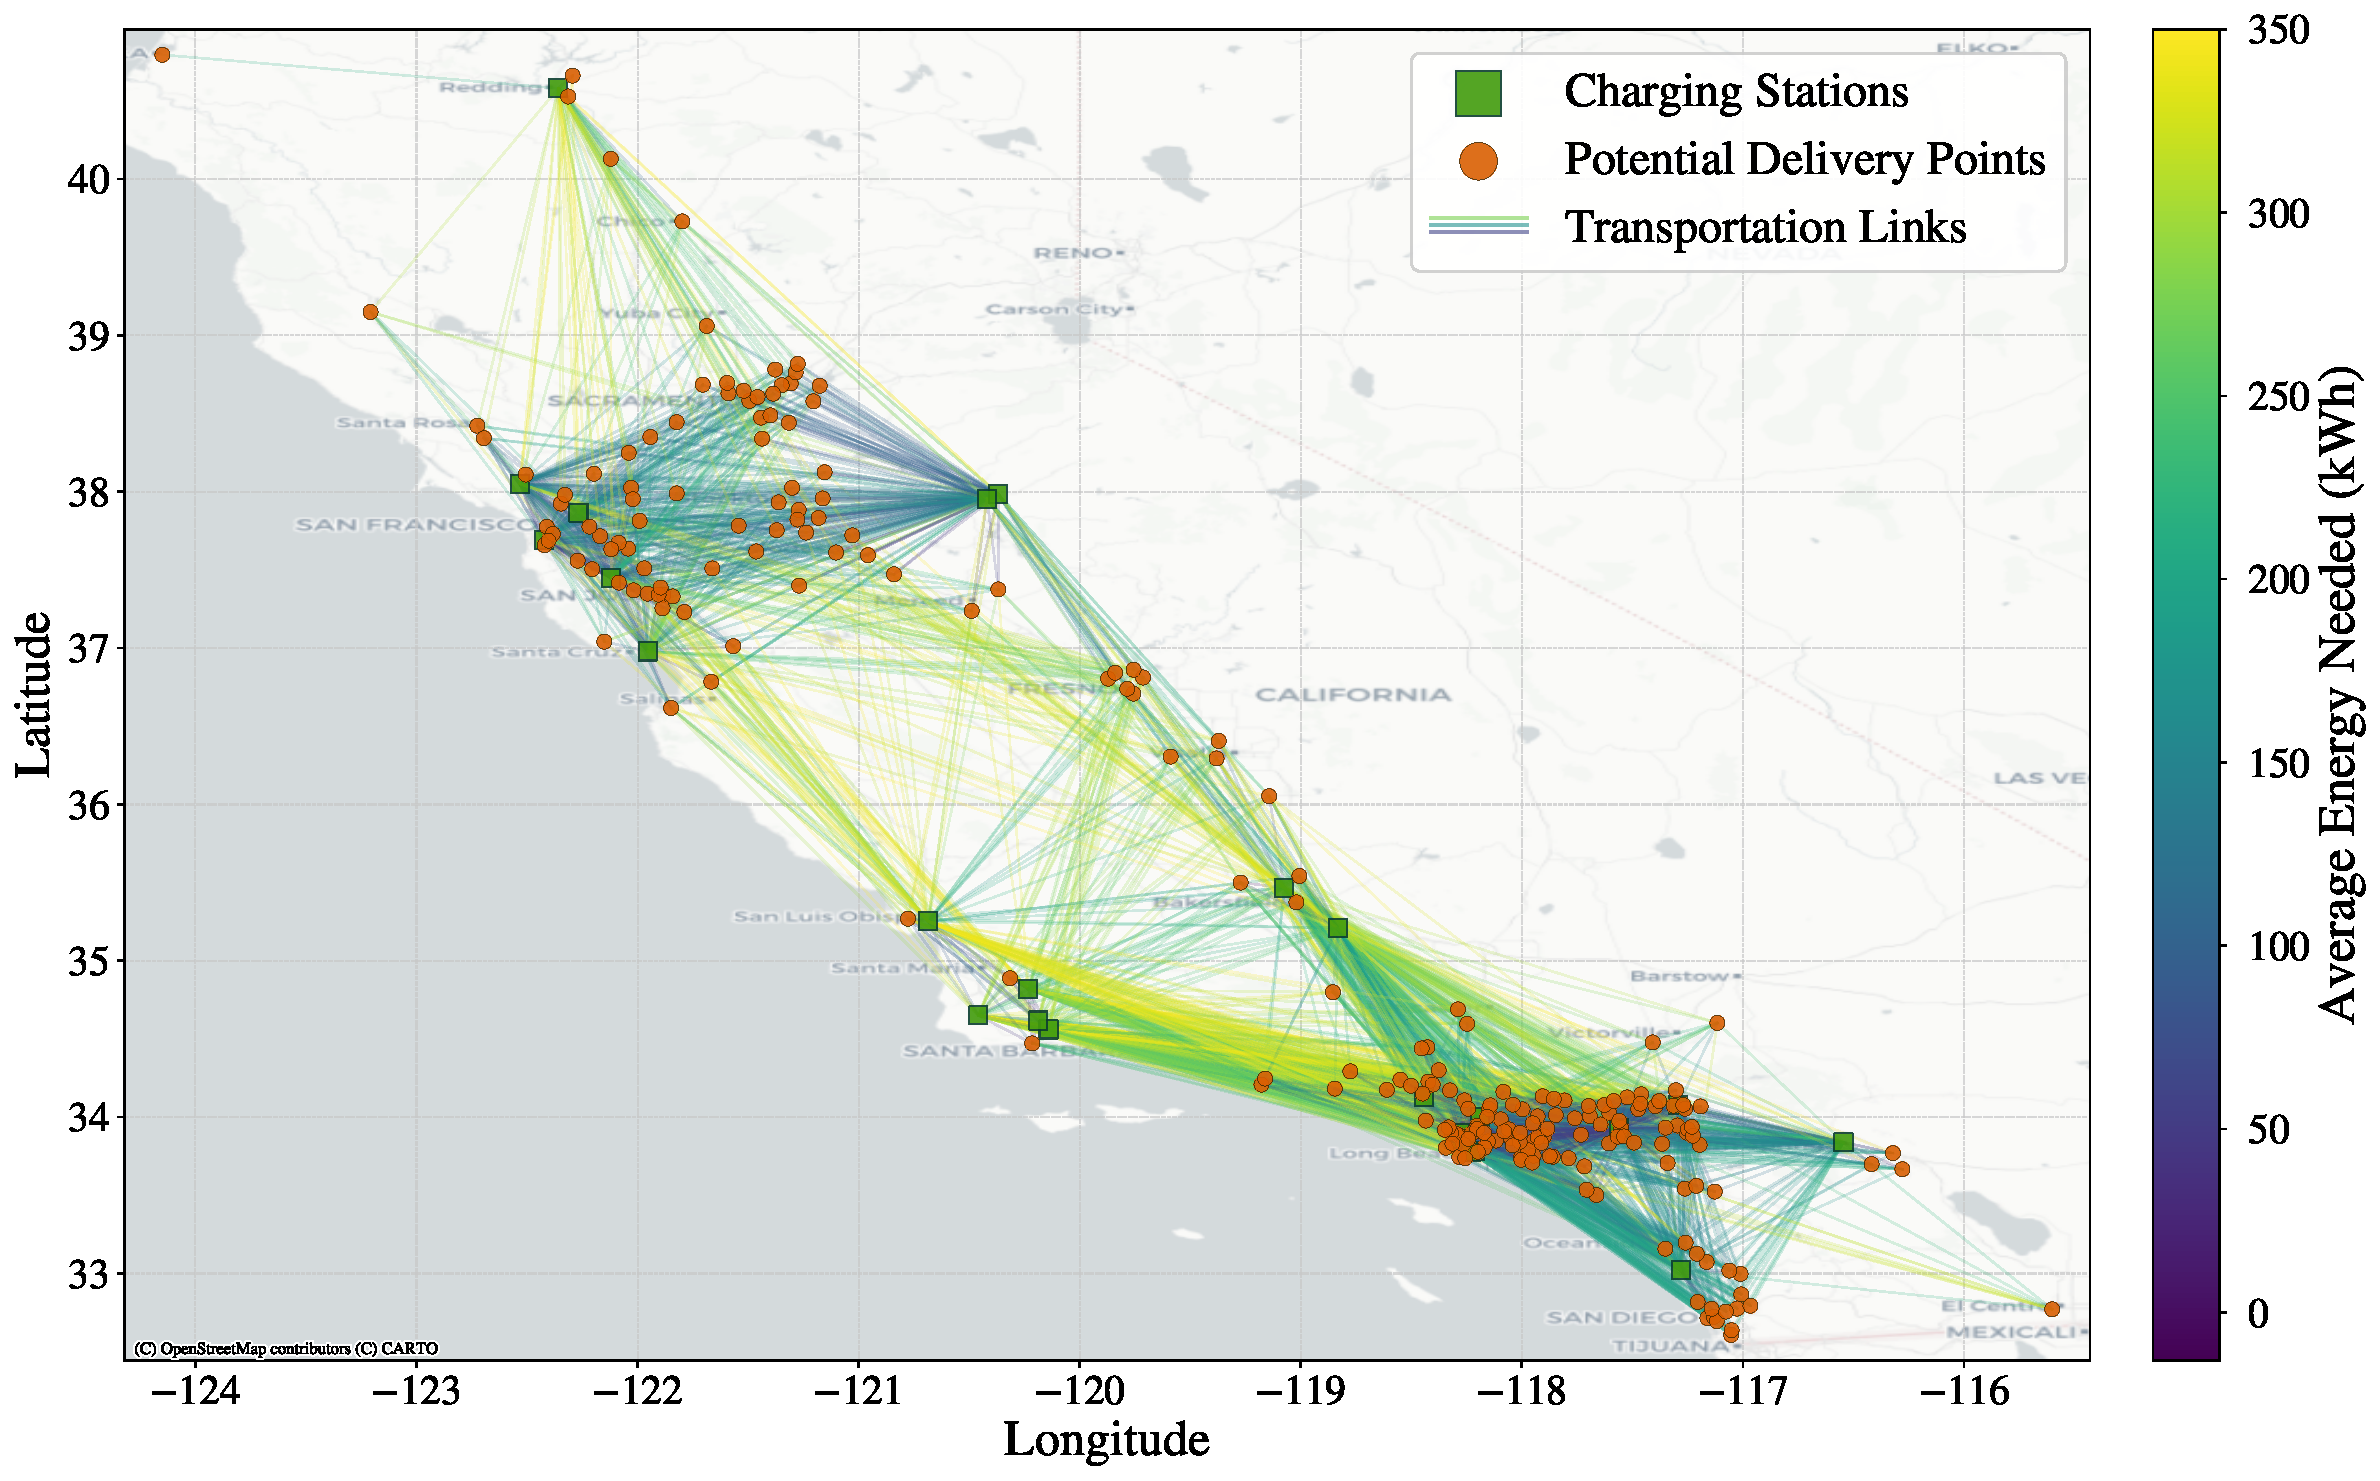
\includegraphics[width=0.75\linewidth]{transport_graph.pdf}
\caption{Experimental transportation network used in the case study. The figure shows the California transportation graph~\cite{ziyan2025} with sampled delivery locations and charging stations overlaid on the map. Node and edge colors indicate the spatial variation in energy and travel conditions across the network.}
\label{fig:cali}
\end{figure}

All reported results are averages over 200 evaluation scenarios, and training is performed with 5 random seeds, over which the reported values are averaged. Seed replication is not a formality here: in the joint setting of Section~\ref{sec:joint_evrp} we measure a spread of $0.107$ in success rate across seeds of an identical configuration, which is larger than several of the effects reported in the literature for this class of method, and we interpret differences accordingly. GraphPPO's feature extractor has 3 graph layers, each with 256 nodes, a critic MLP head with 1 layer and 256 nodes, a learning rate of $3\times10^{-4}$, and a discount factor of $\gamma = 0.99$. For both GraphPPO and the PPO-based baselines, the nominal training budget is $10^6$ environment steps with periodic evaluation during training. 
The generic PPO and MaskPPO baselines use the default Stable-Baselines3~\cite{sb3} configuration, with training requiring approximately 5--6 hours, compared with about 10 hours for the proposed GraphPPO. Although training requires several hours offline, the resulting models can generate high-quality solutions in real time at deployment.
Training is done on a system with an A10 GPU and a 16-core Intel CPU, and 24 GB of RAM. 

The joint fleet eVRP study of Section~\ref{sec:joint_evrp} follows a separate and stricter protocol, which we state here because it governs every number in Sections~\ref{sec:joint_evrp}--\ref{sec:transfer}. Scenario seeds are drawn from provably disjoint train, validation, and test namespaces. All baseline hyperparameters and all checkpoint selections are made on validation scenarios only, under a pre-declared rule, and no test scenario is read until the frozen method set is scored. Ablation arms are re-scored on validation scenarios beyond those used to select their own checkpoints, so a comparison between arms is independent of the selection that produced them. Each evaluated method publishes an immutable manifest recording the resolved configuration, the seed list, the code revision, and the checkpoint, together with per-episode rows that retain failures and record their cause; aggregate figures conditioned on success state the conditioning explicitly.

Two consequences of this protocol should be read alongside the results. First, because independently seeded runs of the identical configuration differ by up to $0.107$ in success rate at the interaction budget used for the ablations, differences smaller than roughly $0.1$ are reported as indistinguishable from training noise rather than interpreted. Learned entries in Table~\ref{tab:joint_evrp_metrics} therefore give a seed range where three seeds were trained and are marked as single-seed otherwise. Second, the optimization baseline used in that study is a fleet-level CP-SAT model whose nominal objective was checked against exhaustive enumeration on instances small enough to enumerate; it agrees with brute force on all of them, as does the ALNS metaheuristic, so the planners' shortfall in the stochastic setting reflects open-loop execution rather than an inability to solve the nominal problem.


\subsection{Performance Across Truck Fleet Scales}

Five routing algorithms are considered in this comparison. Mathematical optimization is used as a high-quality planning reference, obtained by solving the optimization model conservatively, as shown in Section~\ref{sec:obj_constraints}, under the same environment assumptions, but without fully accounting for the problem's stochastic nature.
The heuristic algorithm is a rule-based baseline designed to construct feasible routing and charging decisions with low computational effort but without learning, generic PPO~\cite{ppo} is a widely used on-policy algorithm for discrete action spaces and serves here as the standard method applied without any explicit structural adaptation to the transportation graph or the feasibility structure of the problem, while MaskPPO~\cite{maskppo} augments PPO with an action-feasibility mask so that invalid routing and charging actions are removed during decision making. GraphPPO further extends this idea through graph-based state and action representations that encode interactions among trucks, deliveries, and charging stations under shared infrastructure constraints.

Table~\ref{tab:genresults} summarizes the eTFRP performance across fleet sizes from  1 truck with 3 stops (1T3S) to 100 trucks (100T3S), and Figure~\ref{fig:wr} complements these averages by showing which method achieves the best outcome (referred to as ``win ratio'') on each individual test scenario.
Although each truck completes exactly three delivery stops in this setting, the proposed formulation readily extends to an arbitrary number of stops, as demonstrated in the next section.
Performance is evaluated using normalized reward (relative to the mathematical benchmark) and the scheduling success rate (number of routes completed without any stranded trucks). Therefore, values close to $1.0$ indicate near-benchmark performance, values substantially below $1.0$ indicate a clear performance gap, and values slightly above $1.0$ may still be observed because evaluation is carried out under stochastic simulation over 200 random scenarios, where Math. Opt. provides a conservative solution. Here, all learning algorithms are trained specifically for each problem setting.

A clear separation among methods is reported in Table~\ref{tab:genresults}, with GraphPPO being the only learning-based method for which near-benchmark performance is retained across all settings, since normalized rewards of $0.987$ to $1.005$ are obtained for even the hardest setting with 100 trucks, while the corresponding success rates remain similar to the Math. Opt. solution. In contrast, PPO yields very weak results, with normalized reward ranging from $0.081$ to $0.321$ and success falling to $0\%$ from 5T3S onward. Furthermore, MaskPPO shows the strength of the proposed feasible action mask (shown in Section~\ref{sec:feasible_actions}) with normalized reward from $0.972$ to $0.989$ up to 30T3S, while its robustness is sharply reduced as scale increases, with success declining from $98.0\%$ in 1T3S to $53.0\%$ in 30T3S, $4.5\%$ in 50T3S, and $2.0\%$ in 100T3S. Meanwhile, the heuristic remains competitive only in smaller settings and is reduced to $0\%$ success from 30T3S onward.

\label{sec:general-results}
\begin{table}
\centering
\small
\caption{Performance comparison of optimization, heuristic, and learning-based methods across different eTFRP settings. Each learning-based model was trained specifically for the corresponding eTFRP setting and subsequently evaluated on 200 random scenarios. Entries report normalized reward mean and standard deviation, while the success rate is shown within the parentheses (\%). Bold numbers denote the best normalized reward for each setting.}
\resizebox{1\linewidth}{!}{
\begin{tabular}{@{}lccccc@{}}
\toprule
Setting & Math. Opt. & Heuristic & PPO & MaskPPO & GraphPPO (Ours) \\
\midrule
1T3S & $\mathbf{1.000}$ ($99.5$\%) & $0.806$ $\pm$ $0.448$ ($83.0$\%) & $0.081$ $\pm$ $0.428$ ($15.5$\%) & $0.972$ $\pm$ $0.229$ ($98.0$\%) & $0.987$ $\pm$ $0.136$ ($99.0$\%) \\
5T3S & $\mathbf{1.000}$ ($97.5$\%) & $0.814$ $\pm$ $0.213$ ($42.5$\%) & $0.091$ $\pm$ $0.198$ ($0.0$\%) & $0.980$ $\pm$ $0.085$ ($89.5$\%) & $\mathbf{1.000}$ $\pm$ $0.039$ ($97.0$\%) \\
10T3S & $\mathbf{1.000}$ ($95.5$\%) & $0.803$ $\pm$ $0.150$ ($16.5$\%) & $0.083$ $\pm$ $0.152$ ($0.0$\%) & $0.989$ $\pm$ $0.055$ ($87.5$\%) & $\mathbf{1.000}$ $\pm$ $0.027$ ($95.0$\%) \\
30T3S & $\mathbf{1.000}$ ($88.5$\%) & $0.796$ $\pm$ $0.082$ ($0.0$\%) & $0.125$ $\pm$ $0.086$ ($0.0$\%) & $0.974$ $\pm$ $0.035$ ($53.0$\%) & $0.999$ $\pm$ $0.014$ ($86.5$\%) \\
50T3S & $1.000$ ($77.0$\%) & $0.802$ $\pm$ $0.066$ ($0.0$\%) & $0.305$ $\pm$ $0.090$ ($0.0$\%) & $0.948$ $\pm$ $0.036$ ($4.5$\%) & $\mathbf{1.005}$ $\pm$ $0.013$ ($76.5$\%) \\
100T3S & $1.000$ ($59.5$\%) & $0.800$ $\pm$ $0.048$ ($0.0$\%) & $0.321$ $\pm$ $0.059$ ($0.0$\%) & $0.959$ $\pm$ $0.023$ ($2.0$\%) & $\mathbf{1.005}$ $\pm$ $0.011$ ($60.0$\%) \\
\bottomrule
\end{tabular}
}
\label{tab:genresults}
\end{table}

\begin{figure}
  \centering
  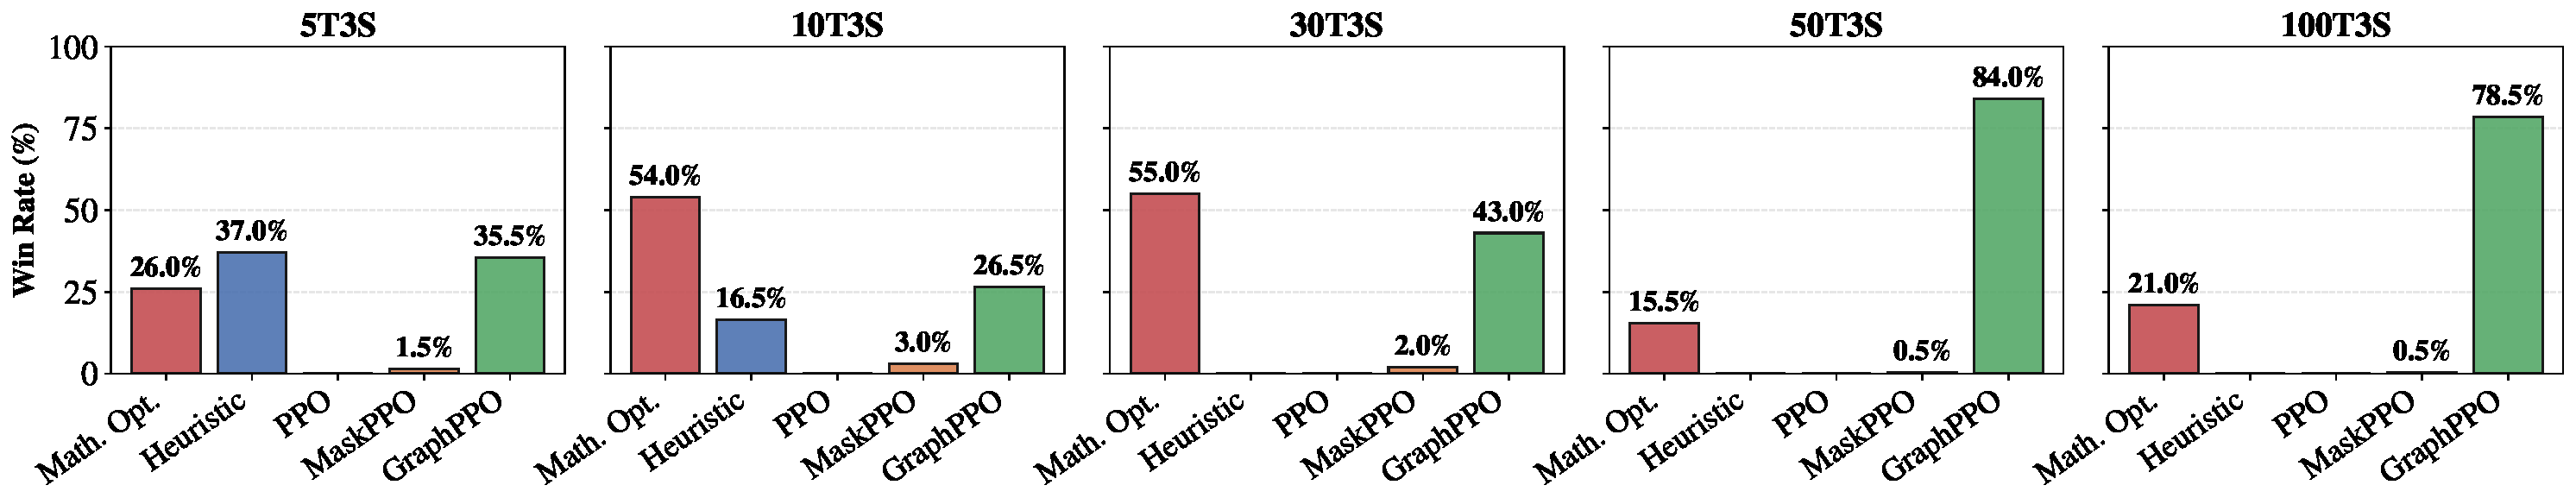
\includegraphics[width=1\linewidth]{win_rates.pdf}
\caption{Comparison of episode-wise winning frequency across 200 simulation episodes for different eTFRP settings. Each bar shows the percentage of episodes in which a method produced the best-performing solution among the compared methods.}
\label{fig:wr}
\end{figure}

Additional results are provided in Figure~\ref{fig:wr} through episode-wise win rates over the 200 evaluation scenarios, where in 5T3S the highest share is attained by the heuristic at $37.0\%$, with GraphPPO close behind at $35.5\%$ and Math.\ Opt.\ at $26.0\%$, while in 10T3S and 30T3S the largest win rates are still recorded for Math.\ Opt.\ at $54.0\%$ and $55.0\%$, with GraphPPO remaining second at $26.5\%$ and $43.0\%$, and in the largest settings a clear shift is observed, since GraphPPO attains $84.0\%$ in 50T3S and $78.5\%$ in 100T3S, compared with only $15.5\%$ and $21.0\%$ for Math.\ Opt., from which it can be inferred that near-benchmark average performance is not only preserved by GraphPPO, but superior competitiveness is also achieved in the most congested large-fleet regimes.




\subsection{Generalization from a Single Training Setting}

\begin{figure} 
\centering
     \subfloat[Normalized reward ratio]{
         \centering
         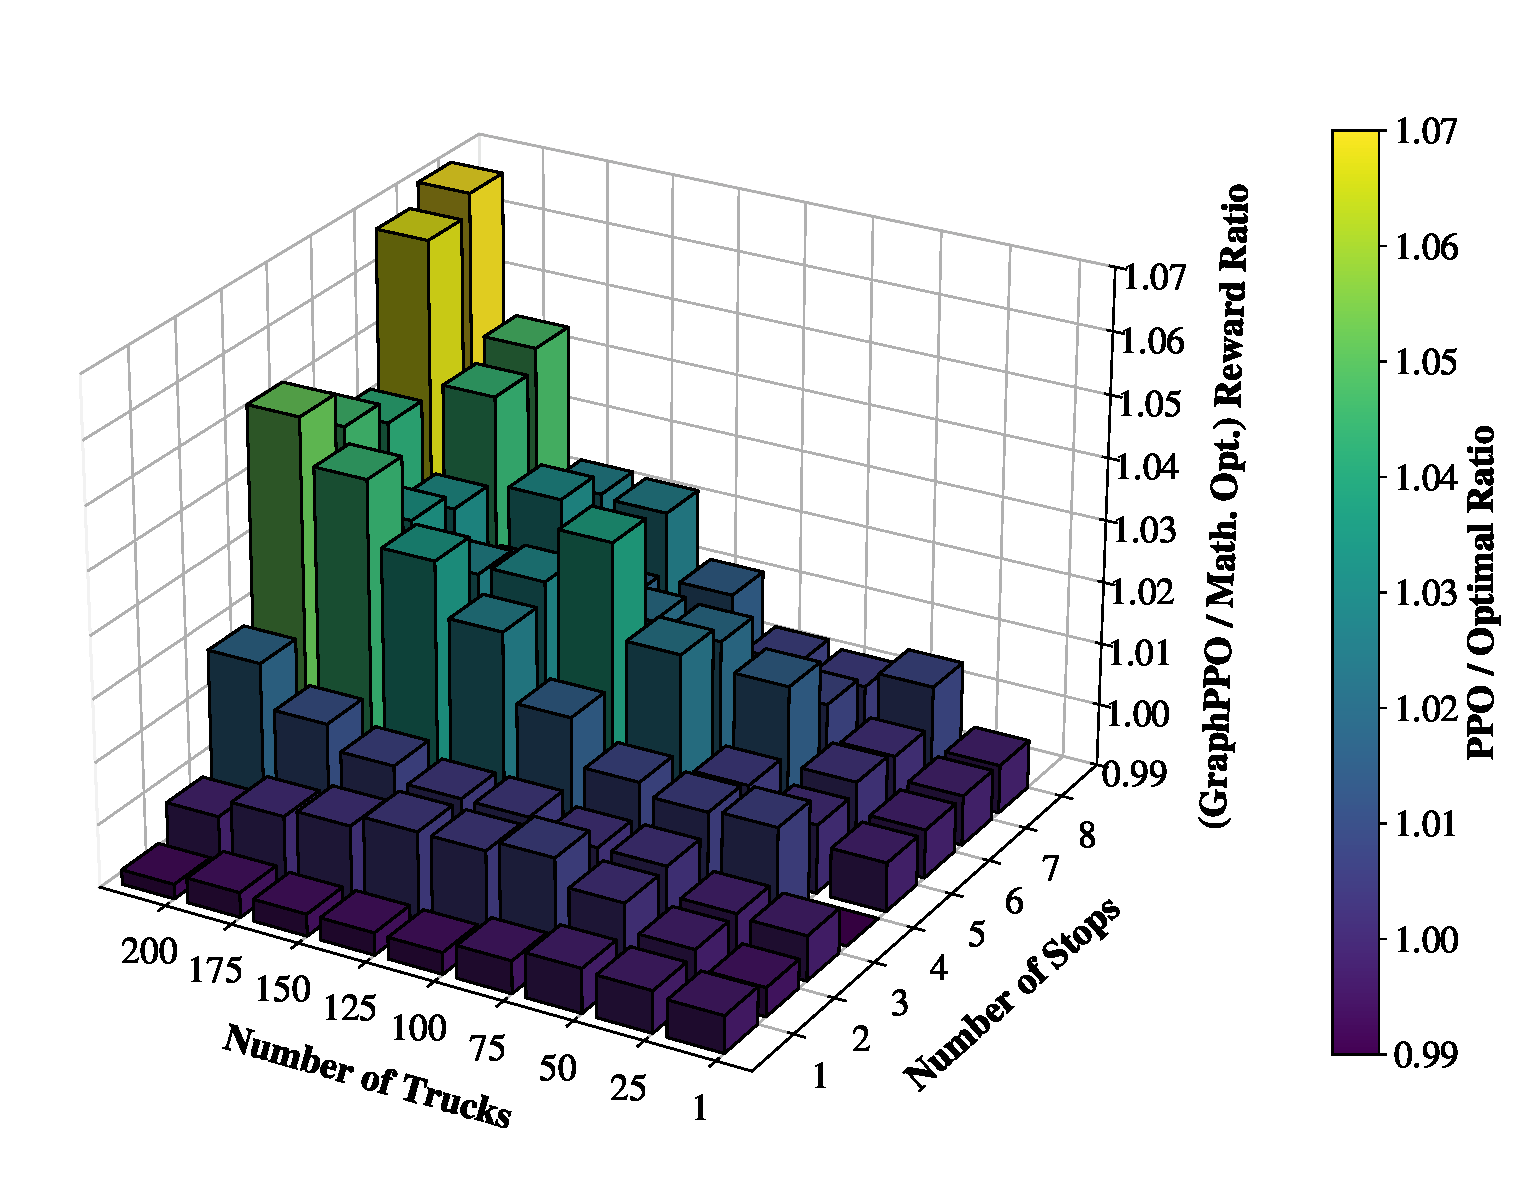
\includegraphics[width=0.4\linewidth]{grid_eval_3d_ratio_plot.pdf}
         \label{fig:gen_a}
         }
        \hspace{10mm}
     \subfloat[Win ratio]{
         \centering
         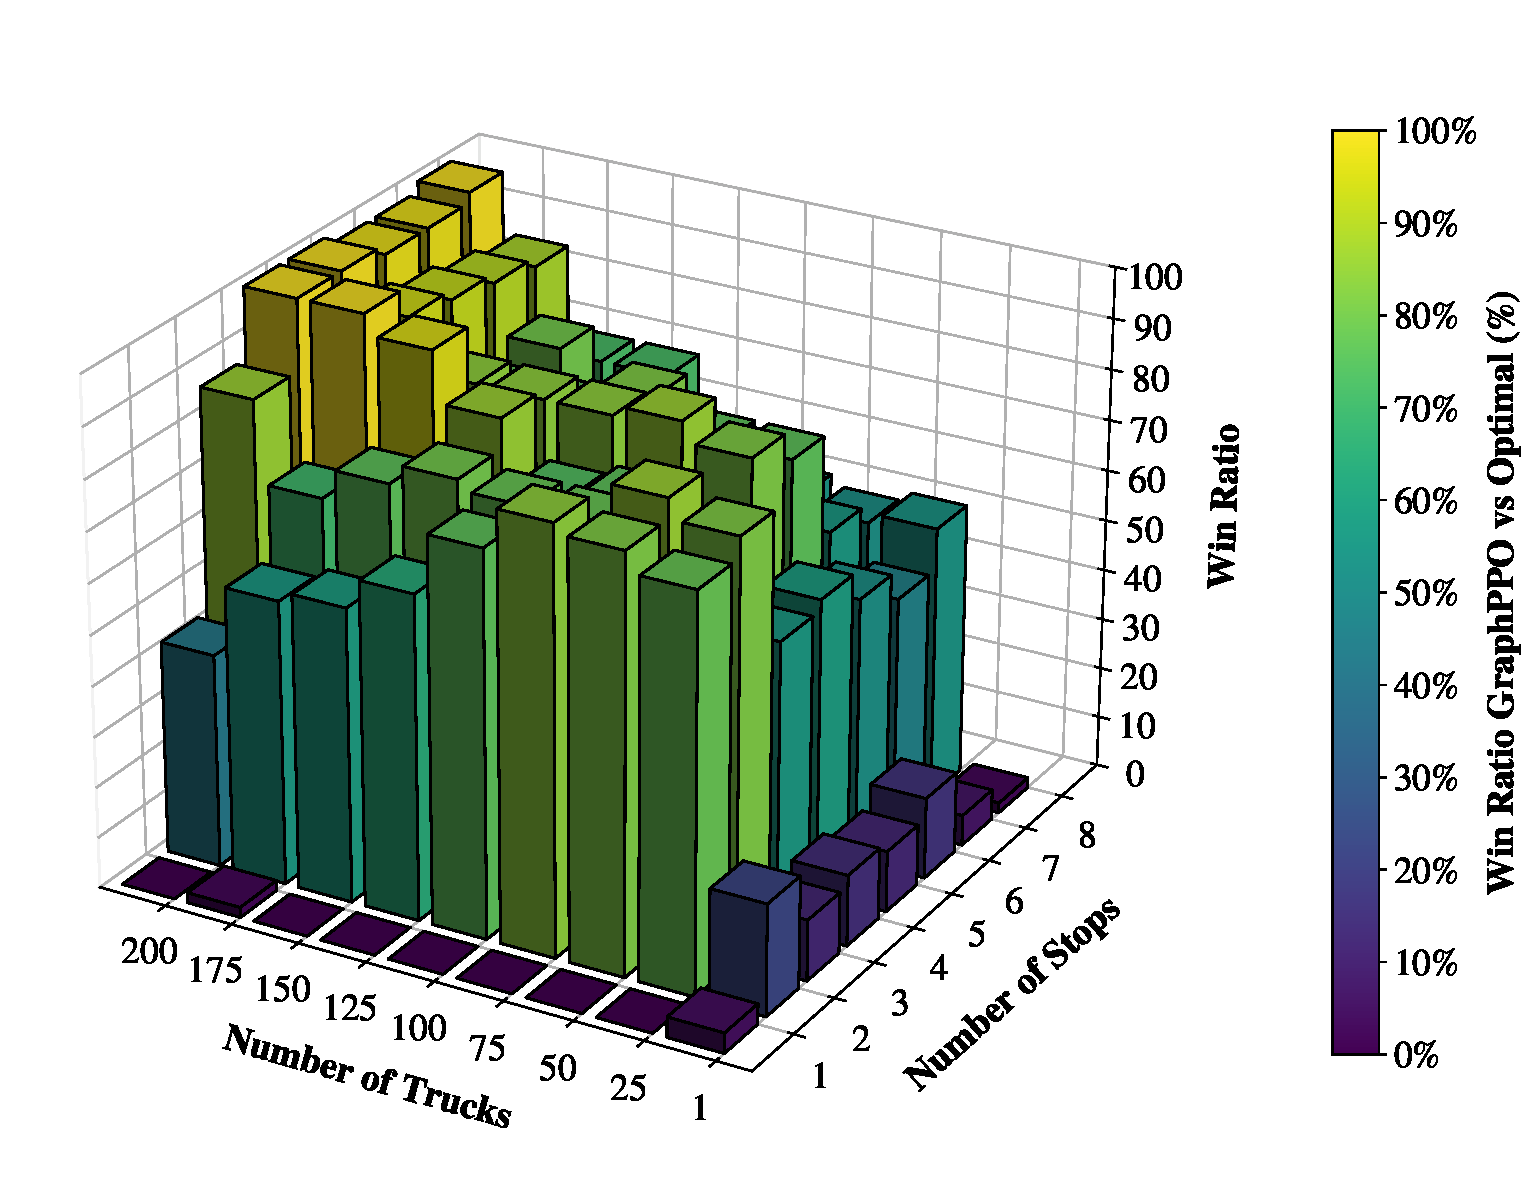
\includegraphics[width=0.4\linewidth]{grid_eval_3d_ratio_plot_win_ratio.pdf}
         \label{fig:gen_b}
         }
    \caption{Generalization performance of a GraphPPO policy trained only on the 100T3S setting and evaluated without retraining across different eTFRP configurations, averaged over 50 random scenarios per case. Panel (a) reports the normalized reward ratio relative to Math.\ Opt., while panel (b) reports the win ratio against Math.\ Opt., defined as the percentage of scenarios in which GraphPPO achieves the better outcome.}
        \label{fig:gen}
\end{figure}


A \emph{size-transfer} analysis is conducted in Figure~\ref{fig:gen}, where a single GraphPPO policy trained only on the 100T3S setting is applied directly to all other fleet-size and stop-count configurations without any retraining or fine-tuning. The transfer examined here is deliberately narrow: the generator, the road network, the vehicle parameters, and the uncertainty law are all held fixed, and only the instance size changes. It is therefore evidence of transfer across scale, not of out-of-distribution generalization; the latter is examined separately in Section~\ref{sec:joint_evrp}, where the charging infrastructure, battery capacity, service times, road distances, and uncertainty distributions are each shifted in turn. The horizontal axes span the number of trucks and the number of sequential stops per truck, while each reported value is averaged over 50 random scenarios. Two complementary metrics are shown. Panel~(a) reports the normalized reward ratio, defined as the average GraphPPO reward divided by the average reward of Math.\ Opt.\ for the same setting, so values above $1.0$ indicate that the transferred policy outperforms the conservative optimization benchmark on average. Panel~(b) reports the win ratio against Math.\ Opt., i.e., the percentage of scenarios in which GraphPPO achieves a better outcome than the optimization benchmark.

Strong transfer performance is observed over a broad region of the test space. In panel~(a), the normalized reward ratio remains very close to or above parity in almost all settings, typically lying around $1.00$ to $1.04$, while the strongest gains are obtained in larger and more congested instances, where values rise to approximately $1.06$ to $1.07$. The largest advantage is visible in high-truck and mid-to-high stop settings, especially around 150 to 200 trucks and roughly 5 to 7 stops, indicating that the policy learned on 100T3S captures decision patterns that remain effective as congestion and fleet interactions become even stronger.
At the same time, only limited degradation is observed in smaller settings. A likely explanation is that instances with few trucks or stops offer relatively little variability in feasible solutions, making the decision landscape simpler. Consequently, the reward ratio remains close to 1.0, suggesting that the learned policy does not over-specialize to the training configuration.

The win-ratio results in panel~(b) further support this conclusion, although a more heterogeneous pattern is observed because this metric is stricter than average reward comparison. For medium and large fleets with approximately 2 to 6 stops, GraphPPO wins in a large majority of scenarios, with win ratios often between $70\%$ and $100\%$, and with the highest values appearing in the dense multi-truck regimes where charger competition is strongest. By contrast, the smallest instances and the one-stop cases are associated with much lower win ratios, in some cases close to zero, indicating that the optimization benchmark remains more competitive when the problem structure is simple, and congestion at charging stations is limited. Overall, the results indicate that the policy trained on 100T3S generalizes well across both smaller and larger eTFRP settings, with the most substantial advantage retained in the operational regimes most relevant to large-scale fleet coordination.




\subsection{In-Depth Analysis for a Single Setting}

A more detailed comparison is provided through the representative 10T3S setting, which corresponds to 10 trucks and 3 sequential delivery stops per truck, while all reported values in Table~\ref{tab:10t3s_metrics} are averaged over 200 evaluation scenarios and are shown as mean $\pm$ standard deviation.

The 10T3S setting is selected as a representative benchmark because it strikes a balance between problem complexity and computational tractability. With 10 trucks and 3 sequential delivery stops per truck, the setting introduces sufficient combinatorial diversity to meaningfully evaluate the model's decision-making capabilities while remaining interpretable for detailed analysis.
Table~\ref{tab:10t3s_metrics} shows detailed results averaged over 200 evaluation scenarios.
The reported {Reward} corresponds to the episodic return used by the environment, which jointly reflects routing, charging, waiting, unloading, successful delivery, and failure penalties. The {Success Rate} indicates the percentage of scenarios completed feasibly. The {Avg.\ Truck SoC at Finish} measures the average remaining battery level at the end of the episode, while {Total Deliveries} reports how many deliveries are completed across the fleet. The charging-related indicators are separated into {Total Charging Sessions}, which counts the number of charging actions; {Total Charging Time}, which measures the aggregate time spent charging, and {Total Waiting Time}, which captures the time spent in charger queues. In addition, {Total Routing Time} and {Unloading Time} quantify time spent traveling and servicing deliveries, {Total Time} summarizes the overall operational duration, and Exec.\ Time reports the wall-clock solution time required by each method.


\begin{table}
\centering
\small
\caption{Detailed metric performance comparison for the 10T3S setting over 200 evaluation scenarios. Reported values are the mean and standard deviation over the evaluation scenarios.}
\begin{tabular}{@{}lccccc@{}}
\toprule
Metric & Math. Opt. & Heuristic & PPO & MaskPPO & GraphPPO (Ours) \\
\midrule
Reward (-) & $14582$ $\pm$ $583$ & $11718$ $\pm$ $2245$ & $1244$ $\pm$ $2205$ & $14404$ $\pm$ $721$ & $14574$ $\pm$ $568$ \\
Success Rate (\%) & $95.5$ $\pm$ $20.8$ & $16.5$ $\pm$ $37.2$ & $0.0$ $\pm$ $0.0$ & $87.5$ $\pm$ $33.2$ & $95.0$ $\pm$ $21.8$ \\
Avg. Truck SoC at Finish (\%) & $36.0$ $\pm$ $3.4$ & $14.6$ $\pm$ $6.4$ & $27.0$ $\pm$ $6.4$ & $50.1$ $\pm$ $7.1$ & $14.2$ $\pm$ $2.4$ \\
Total Deliveries (-) & $29.9$ $\pm$ $0.7$ & $27.4$ $\pm$ $2.2$ & $19.4$ $\pm$ $2.3$ & $29.7$ $\pm$ $0.9$ & $29.9$ $\pm$ $0.6$ \\
Total Charging Sessions (-) & $13.5$ $\pm$ $1.8$ & $9.2$ $\pm$ $2.0$ & $0.0$ $\pm$ $0.0$ & $11.4$ $\pm$ $5.3$ & $13.5$ $\pm$ $2.6$ \\
\midrule
Total Charging Time (H) & $63.1$ $\pm$ $10.0$ & $28.4$ $\pm$ $7.7$ & $0.0$ $\pm$ $0.0$ & $87.8$ $\pm$ $19.0$ & $48.6$ $\pm$ $12.3$ \\
Total Waiting Time (H) & $4.3$ $\pm$ $8.2$ & $0.7$ $\pm$ $2.0$ & $0.0$ $\pm$ $0.0$ & $5.4$ $\pm$ $9.0$ & $2.0$ $\pm$ $3.7$ \\
Total Routing Time (H) & $224.3$ $\pm$ $16.6$ & $207.8$ $\pm$ $20.3$ & $132.5$ $\pm$ $12.7$ & $246.7$ $\pm$ $29.6$ & $249.6$ $\pm$ $23.2$ \\
Unloading Time (H)& $4.0$ $\pm$ $0.1$ & $3.8$ $\pm$ $0.2$ & $3.5$ $\pm$ $0.3$ & $4.0$ $\pm$ $0.1$ & $4.0$ $\pm$ $0.1$ \\
Total Time (H) & $295.8$ $\pm$ $27.3$ & $240.7$ $\pm$ $26.9$ & $136.0$ $\pm$ $12.9$ & $343.9$ $\pm$ $48.0$ & $304.1$ $\pm$ $35.0$ \\
\midrule
Exec. Time (s) & $1.9$ $\pm$ $0.7$ & $0.1$ $\pm$ $0.1$ & $0.2$ $\pm$ $0.2$ & $1.0$ $\pm$ $0.7$ & $1.7$ $\pm$ $0.3$ \\
\bottomrule
\end{tabular}
\label{tab:10t3s_metrics}
\end{table}

For this case, near-equivalence between GraphPPO and the mathematical benchmark is observed in the two most important outcome metrics. A reward of $14574$ is obtained by GraphPPO, compared with $14582$ for Math.\ Opt., while the success rate remains almost identical at $95.0$ versus $95.5$. A comparable number of deliveries is also completed, with both methods averaging $29.9$ deliveries, and an identical average number of charging sessions is recorded at $13.5$. These results indicate that the proposed policy reproduces the overall quality and feasibility of the optimization benchmark under stochastic execution. By contrast, substantial degradation is observed for the heuristic and PPO baselines. The heuristic reaches a reward of $11718$ with only $16.5\%$ success, while generic PPO collapses completely with $0.0\%$ success and only $19.4$ completed deliveries. MaskPPO remains much stronger than PPO, with a reward of $14404$ and success of $87.5\%$, but still remains below both Math.\ Opt.\ and GraphPPO in reliability.

The operational metrics further clarify the behavioral differences among methods. GraphPPO ends with a lower residual SoC than Math. Opt.\ at $14.2\%$ versus $36.0\%$, which suggests that less conservative battery utilization is being adopted while feasibility is still preserved. This behavior is also reflected in the charging profile, since GraphPPO spends only $48.6$ hours in charging compared with $63.1$ for Math. Opt., and queueing time is reduced from $4.3$ hours to $2.0$ h. At the same time, a longer routing time is observed for GraphPPO at $249.6$ hours versus $224.3$, so the final total time is slightly higher at $304.1$ hours compared with $295.8$. A different pattern is observed for MaskPPO, where a very high terminal SoC of $50.1\%$ is retained together with $87.8$ hours of charging time and $343.9$ hours of total time, indicating an overly conservative charging strategy. Finally, low online solution times are maintained by all methods, with $1.7$ seconds for GraphPPO and $1.9$ seconds for Math.\ Opt. (since there are only 10 trucks), while the heuristic and PPO-based baselines remain below one second, so near-real-time deployment remains feasible for the proposed policy in this setting.

\subsection{From eTFRP to Joint Fleet eVRP}\label{sec:joint_evrp}

The preceding subsections assess the eTFRP, in which delivery points are assigned to trucks in advance and the fleet competes for shared charging infrastructure. That formulation reflects the operational reality this work targets, where assignments follow from contracts and depot logistics rather than being chosen by the routing system. It does, however, leave open whether the proposed representation depends on that structure. To test this, a second and deliberately harder setting is introduced in which the decisions removed by the eTFRP are restored: customers are owned by the fleet rather than pre-assigned, assignment and sequencing are decided online, payload capacity binds, and every truck must return to the depot. This joint fleet eVRP is solved by the same architecture without modification.

The objective in this setting is total fleet travel time on a plan that serves every customer, and the evaluation is feasibility-first: a plan that abandons deliveries is worthless however short its tour, so the success rate dominates and travel time only breaks ties. All methods are scored on the same 500 held-out scenarios, and the learned rows report the mean over three independent training seeds where available. The optimization benchmark is a fleet-level CP-SAT model over the nominal network, executed with energy-safe repair, whose objective was validated against exhaustive enumeration on tiny instances; an adaptive large neighbourhood search (ALNS) over the same nominal costs is included as a strong metaheuristic, and it reaches the enumerated optimum on every instance small enough to enumerate.

\begin{table}
\centering
\small
\caption{Performance comparison for the joint fleet eVRP setting over 500 held-out evaluation scenarios, in which assignment, sequencing, charging, and depot return are all decided online. GraphPPO reports the mean over three independent training seeds with the seed range in brackets; all other learning-based rows are single seeds trained at a smaller interaction budget. As in the eTFRP tables, PPO denotes a flat-state policy with independent action scoring and no feasibility mask, and MaskPPO the same policy with the hard mask; DeepSets-PPO, the state-GNN, and the attention model are reported in the text rather than as further columns. Travel, charging, service, and total times are fleet totals averaged over all episodes, so a method that declines instances is not flattered by conditioning.}
\begin{tabular}{@{}lcccccc@{}}
\toprule
Metric & CP-SAT & ALNS & Heuristic & PPO & MaskPPO & GraphPPO (Ours) \\
\midrule
Success rate (\%) & $62.2$ & $61.4$ & $55.2$ & $45.2$ & $50.6$ & $\mathbf{84.3}$ $[83.0, 85.8]$ \\
Wilson 95\% CI & $[57.9, 66.3]$ & $[57.1, 65.6]$ & $[50.8, 59.5]$ & $[40.9, 49.6]$ & $[46.2, 55.0]$ & $[79.5, 88.6]$ \\
Completed fraction (-) & $0.932$ & $0.930$ & $0.917$ & $0.960$ & $0.968$ & $\mathbf{0.991}$ \\
Avg.\ truck SoC at finish (\%) & $56$ & $57$ & $62$ & $40$ & $46$ & $49$ \\
Total charging sessions (-) & $34.6$ & $35.4$ & $44.4$ & $16.2$ & $18.9$ & $\mathbf{13.4}$ \\
\midrule
Total charging time (H) & $15.6$ & $15.7$ & $19.4$ & $10.7$ & $11.2$ & $\mathbf{9.4}$ \\
Total routing time (H) & $167.5$ & $168.6$ & $199.8$ & $136.6$ & $143.1$ & $\mathbf{123.5}$ $[120.9, 125.3]$ \\
Unloading time (H) & $1.9$ & $1.9$ & $1.9$ & $2.0$ & $2.0$ & $2.0$ \\
Total time (H) & $184.9$ & $186.3$ & $221.1$ & $149.2$ & $156.3$ & $\mathbf{134.8}$ \\
\midrule
Exec.\ time (ms/decision) & $2.4$ & $2.0$ & $\mathbf{0.8}$ & $1.9$ & $1.9$ & $5.6$ \\
\bottomrule
\end{tabular}
\label{tab:joint_evrp_metrics}
\end{table}

As shown in Table~\ref{tab:joint_evrp_metrics}, the ordering observed in the eTFRP is preserved when the combinatorial decisions are restored, but the margin is obtained on a different axis. A success rate of $84.3\%$ is achieved by GraphPPO, against $62.2\%$ for CP-SAT and $61.4\%$ for ALNS, a difference of more than twenty percentage points whose Wilson intervals are disjoint. The two search-based planners agree closely with one another, which is expected given that both solve the same nominal problem and both match exhaustive enumeration where enumeration is possible; their shortfall is therefore not a failure of search but of open-loop execution under realized travel times, energy draws, and service durations.

Because methods decline different instances, their conditional means are not directly comparable, and a paired reading on jointly solved scenarios is required. On the $285$ scenarios solved by both, GraphPPO and CP-SAT differ by $+0.2$ hours of fleet travel time with a $95\%$ confidence interval of $[-3.1, +3.7]$, and GraphPPO wins $53\%$ of the head-to-head comparisons; against ALNS the difference is $+0.9$ hours $[-2.5, +4.4]$. The proposed method is therefore statistically indistinguishable from a validated exact planner on the campaign objective while completing substantially more instances. Against the remaining baselines the differences are unambiguous: $-23.0$ hours $[-26.7, -19.1]$ against the heuristic and $-26.1$ hours $[-29.7, -22.3]$ against the rolling-horizon controller. The remaining learned baselines, omitted from the table for width, sit between the two extremes: DeepSets-PPO reaches $67.0\%$ success at $152.3$ travel hours, the state-GNN with independent action scoring $61.2\%$ at $141.0$, and the constructive attention model $78.8\%$ at $144.5$. The attention model is the strongest of them, and at the matched interaction budget it is statistically indistinguishable from the proposed encoder, which is why the state encoder is not claimed as the source of the advantage.

The operational metrics indicate where the advantage originates. The planners build short nominal tours, reflected in their competitive makespans, but sustain them with $34.6$ and $35.4$ charging sessions and $15.6$ to $15.7$ hours of charging, and they abandon roughly four instances in ten when execution departs from the plan. GraphPPO completes $99.1\%$ of deliveries using $13.4$ charging sessions and $9.4$ hours of charging, and its total operating time of $134.8$ hours is $27\%$ below the planners'. A conservative energy policy is retained, with an average terminal state of charge of $49\%$, but it is achieved with fewer and better-placed charging stops rather than with additional ones.

A computational caveat should be stated plainly. In this setting the nominal model is small enough that CP-SAT proves optimality in milliseconds, and its solution is unchanged whether it is given a half-second or forty-five seconds. The order-of-magnitude runtime advantage reported for the single-vehicle case therefore does not carry over here: GraphPPO requires $5.6$~ms per decision against $2.4$~ms for CP-SAT. The argument for the learned policy in this setting rests on solution quality under uncertainty, not on computation time.

\subsection{Ablation and Sensitivity Analysis}\label{sec:ablation}

The joint setting is also used to isolate which components of the proposed representation are responsible for its behaviour. Each arm below modifies exactly one element while holding the observation width, network shape, interaction budget, curriculum, reward, and seed stream fixed, and each is re-scored on validation scenarios disjoint from those used to select its checkpoint. Because independently seeded runs of the identical configuration span $0.107$ in success rate at this budget, effects smaller than roughly $0.1$ are not separable from training noise, and are reported as such rather than interpreted.

Three elements are found to carry the model. Removing the per-action routing features, which price the leg a candidate commits to and the return leg it implies, reduces the success rate from the $0.700$--$0.807$ seed band to $0.213$. Removing the typed pairwise relations between trucks, customers, and chargers reduces it to $0.633$, and withholding the pooled fleet embedding from the action head reduces it to $0.667$. Two elements are found to be inert: blanking the charging-queue state leaves the model at $0.793$ and blanking the active-truck indicator leaves it at $0.727$, both within the seed band. The queue result is a property of the evaluated instances rather than of the architecture, since two trucks distributed over twenty-five stations rarely contend for ports; a congestion-specific study is therefore required before any claim about queue-aware behaviour is made.

The role of the feasibility mask is examined directly, since it is the component most often assumed to explain the performance of masked policies. A variant is trained in which the mask is replaced by one that hides only action slots denoting no action at all, leaving the observation and candidate set unchanged, so that the policy must learn feasibility from experience. Across three seeds per arm, the masked and unmasked variants reach mean success rates of $0.760$ and $0.773$ respectively, with overlapping ranges: at this budget the hard mask is not what produces feasibility, and the unmasked policy averages $0.1$ invalid actions per episode. What proves necessary is that infeasibility carry a cost commensurate with failure. When an infeasible action is merely refused at a tenth of the failure penalty, the policy never learns feasibility at all and the success rate collapses to zero; when the same refusal is charged at the failure penalty, the arm recovers to $0.773$. The mask is best understood as a convenience that supplies this cost for free, rather than as the source of the reported behaviour.

The same ablation was repeated in a pre-assigned variant of the problem, in which customers are bound to
trucks before the episode begins as they are in the eTFRP benchmark, so that only sequencing, charging and routing
remain to be decided. Across two seeds per arm the masked and unmasked policies reach $0.340$ and $0.330$ mean
success, against per-arm seed ranges of $0.054$ and $0.034$: the conclusion is unchanged in the setting the main
benchmark uses. This also locates what the earlier PPO-versus-MaskPPO comparison measures. Those two baselines differ
in their action representation as well as in masking, so their gap is evidence for the structured action space rather
than for the mask specifically.

A second observation from that variant is worth recording because it runs against intuition. At an identical budget
and architecture the same model reaches $0.70$--$0.81$ success when it also decides the assignment, and only
$0.31$--$0.37$ when the assignment is fixed. Removing a decision did not make the problem easier: under
pre-assignment a truck must serve its own customers wherever they fall, so the fleet cannot rebalance when one truck
draws a distant or energy-expensive set, and a customer that becomes unreachable stays unreachable. Assignment is not
only a decision the eTFRP removes; it is also the mechanism by which the joint formulation recovers from an adverse
draw.

The charging action space is examined in the same way. Refining the target state-of-charge grid from $10\%$ to $5\%$ leaves the model inside its seed band, so the coarser discretization is not a binding approximation. Expressing the charging decision as a duration of $15$, $30$, or $60$ minutes instead of a target state of charge reduces success to $0.627$ and increases fleet travel time to $159.3$ hours, placing it outside the band on both axes. The explanation is structural: a fixed duration delivers different amounts of energy depending on the truck's position on the charging curve, so the same action denotes different outcomes in different states, whereas a target state of charge is state-independent by construction.

\subsection{Transfer Beyond the Training Distribution}\label{sec:transfer}

Transfer is assessed on twenty regimes, each scoring every method on identical held-out scenarios, and each labelled as interpolation, within-simulator size transfer, or genuine distribution shift so that evidence of one kind is not quoted as evidence of another. Size transfer is strong: success rates of $0.91$, $0.89$, and $0.81$ are obtained at four, six, and eight customers against a ten-customer training distribution, and $0.72$ with a single truck. The ranking is also preserved under shifts in charger power, charger efficiency, port availability, travel-time variance, energy-draw variance, demand, and a road network whose legs are uniformly $25\%$ faster or $40\%$ slower, with GraphPPO leading thirteen of the sixteen regimes scored for all methods, usually by more than twenty points.

Three regimes reverse the ranking, and they share a mechanism. With a $300$~kWh battery the learned policy reaches $0.34$ against CP-SAT's $0.43$; with a $500$~kWh battery it reaches $0.87$ against $0.98$; and with service times doubled it reaches $0.46$ against ALNS's $0.60$. Each of these shifts the feasibility frontier itself rather than the cost of an individual decision. A planner re-solves against whatever budget it is given, whereas a policy has internalised where that frontier lies and is systematically miscalibrated when it moves. The large-battery case is the clearest: when the problem becomes easy the planners solve almost every instance and the policy does not, because slack it never encountered during training is not exploited. Averaged over the out-of-distribution regimes, the success rate changes by $-0.110$ for GraphPPO against $-0.006$ for ALNS and $+0.009$ for CP-SAT. The learned policy therefore purchases a large in-distribution advantage and returns part of it under distribution shift, with the loss concentrated where the resource budget changes.

\section{Conclusion}

This paper introduced a truck-oriented, learning-compatible framework for the eTFRP and eVRP under charging constraints, nonlinear charging behavior, and operational uncertainty. The problem was formulated as an event-driven semi-Markov decision process with shared charging resources, stochastic travel and energy consumption, and feasibility-aware decision-making, and solved using the proposed GraphPPO method. Across the main multi-truck benchmark, GraphPPO remained consistently close to the mathematical programming baseline, achieving normalized rewards of 0.987--1.005 from 1 to 100 truck instances, while maintaining high success rates even when fleet size increased. By contrast, generic PPO and the heuristics failed almost completely beyond the smallest setting, and MaskPPO, although much stronger than PPO, lost reliability at larger scales. The detailed fleet-level analysis further showed that GraphPPO matched the optimization benchmark not only in reward and deliveries completed, but also through more effective charging behavior, including lower charging and waiting times than MaskPPO under shared infrastructure. In an additional joint fleet eVRP setting, in which customer assignment, sequencing, and a mandatory depot return were restored as online decisions, the same architecture completed $84.3\%$ of instances against $62.2\%$ for a CP-SAT planner whose objective was validated against exhaustive enumeration, while remaining statistically indistinguishable from that planner on fleet travel time. This indicates that the value of the approach extends beyond fleet-level congestion management to the underlying combinatorial routing problem itself.

Two findings qualify these results and are reported because they bound what the method should be claimed to do. First, an ablation in which the feasibility mask is replaced by one that hides only undefined action slots reaches the same success rate as the masked policy across three training seeds, so the mask is a convenience rather than the source of the reported feasibility; what is necessary is that infeasible actions carry a cost commensurate with failure. Second, transfer holds across instance size and most parameter shifts but degrades where the energy or time budget itself moves, and in those regimes a re-solving planner is the stronger choice. Taken together, these results show that the combination of graph-based state--action modeling and explicit feasibility-aware action selection provides a practical approach to electric truck routing in operationally realistic settings, with a clearly identified boundary. 

Several directions for future research follow naturally from this work. First, the current benchmark could be extended to more complex service constraints such as time windows and depot return policies. Second, the interaction between routing and charging could be modeled more deeply by incorporating reservation policies, electricity prices, larger charger heterogeneity, and explicit grid constraints, thereby advancing integrated logistics-energy decision-making. 
Finally, the degradation observed under shifts of the energy and time budget suggests that budget-conditioned training, or an explicit feasibility model learned alongside the policy, may be required before such methods can be deployed across heterogeneous fleets without retraining. 
Such extensions would further strengthen the role of learning-based methods as decision-support tools for real-world electric freight operations. 

% \section*{Acknowledgements}
% The study was funded by the DriVe2X research and innovation project of the European Commission, grant number 101056934. This work also used the Dutch national e-infrastructure, with support from the SURF Cooperative, under grant no. EINF-5716.

% \printcredits

%% Loading bibliography style file
%\bibliographystyle{model1-num-names}
% \bibliographystyle{cas-model2-names}

\appendix

\section{Baseline Specifications and Information Assumptions}\label{app:baselines}

This appendix states what each non-learning baseline knows, what it assumes, and
what it does when its plan fails, so that the comparison in
Section~\ref{sec:joint_evrp} can be reproduced or disputed on its details rather
than on its summary.

\subsection*{A.1 Information available to every method}

All methods, learned and classical, observe the same state: the position,
battery, remaining payload and status of every truck; the location, demand and
service status of every customer; the location, power, port count, occupancy and
waiting list of every station; and the nominal travel time and energy of every
network transition. No method observes a realized travel time, energy draw or
service duration before it is incurred, and no method observes another truck's
future decisions. The nominal network is the same table for all methods and is
never perturbed by the realizations drawn during an episode.

\subsection*{A.2 Greedy heuristic}

The heuristic is goal-directed rather than myopic, and three properties were
necessary to make it a fair opponent rather than a straw man; each is stated
because each corresponds to a failure mode we measured.

\begin{enumerate}[leftmargin=*,nosep]
\item \textbf{Charger choice must close distance to the goal.} Selecting the
nearest station makes trucks shuttle between two adjacent stations indefinitely
when a customer lies more than one battery away.
\item \textbf{A stop is only taken if the truck can also leave it.} Serving a
customer the truck cannot depart from strands it, because the episode requires a
depot return.
\item \textbf{Customers claimed by another truck are excluded.} They are
permanently infeasible for this truck, and targeting them wastes decisions.
\end{enumerate}

\noindent The resulting policy is, at each decision point for the active truck
$i$ at node $n_i$:

\begin{quote}
\small
\textbf{if} a delivery is in progress or the truck must leave a charger:
  take the forced transition.\\
\textbf{else} let $G$ be the set of unserved customers claimable by $i$ within
its remaining payload, plus the depot if all customers are served.\\
\quad Choose the goal $g\in G$ minimising
$\tau_{n_i g} + w\cdot d_g$, where $d_g$ is the customer's demand and $w$ the
demand weight.\\
\quad \textbf{if} $\alpha\cdot b_{n_i g} \le$ battery and the truck can also
leave $g$: drive to $g$.\\
\quad \textbf{else} choose the station $c$ minimising
$\tau_{n_i c} + \tau_{c g}$ among stations reachable with the energy margin
$\alpha$, and drive to $c$; on arrival, charge to the target state of charge.
\end{quote}

\noindent Here $\alpha$ is the energy safety factor. Recharge duration is priced
with the same nonlinear charging routine the simulator executes, not with an
energy-over-power approximation, so the heuristic never plans a recharge the
simulator will not deliver. Parameters ($\alpha$, target state of charge, demand
weight) are grid-searched on validation scenarios only.

\subsection*{A.3 Rolling-horizon controller}

The controller enumerates sequences of the next $H$ stops with branching factor
$B$ over the nominal network, scores each by its nominal completion time with
energy-safe recharges inserted, commits only the first stop, and re-plans at the
next decision point. It is therefore deterministic and receding-horizon: it uses
expected values for travel and energy and never samples scenarios. It executes
through the heuristic's navigation layer, so a failure to reach a planned stop
is repaired rather than propagated.

\subsection*{A.4 CP-SAT planner}

The planner solves the nominal deterministic problem once per scenario: a
circuit formulation per truck over the depot and all unserved customers, with
payload capacity enforced, arc costs equal to nominal travel time plus the
recharge time that arc's energy implies at an average charging power, and an
objective of either the longest route or the sum of routes. It is offline and
deterministic; it does not model queueing, does not sample realizations, and
does not re-solve when execution departs from the plan. Execution uses the same
energy-safe navigation layer, and every episode records how often the plan ran
out and the executor chose instead.

Two properties matter for interpreting the results. First, the circuit admits an
empty route, so a truck may be left idle; without this the model is forced to
use every vehicle and returns strictly worse plans while reporting them as
optimal. Second, the objective is validated: on instances small enough to
enumerate, the solved objective matches exhaustive enumeration over all
assignments and orderings.

\subsection*{A.5 Adaptive large neighbourhood search}

ALNS searches the same nominal objective as the CP-SAT planner. It begins from a
cheapest-insertion construction and repeats: remove a fraction of customers with
one of four destroy operators (random, worst-cost, Shaw-related, whole-route),
reinsert them with greedy or regret-2 insertion, and accept by a
simulated-annealing criterion. Operator weights adapt on the standard
Ropke--Pisinger schedule. The search is deterministic given its seed, and it
executes through the same navigation layer as the other planners. It reports no
optimality bound by construction.

\section{Formulation Assumptions}\label{app:assumptions}

\begin{description}[leftmargin=*,nosep]
\item[Queueing.] Stations admit trucks first-come-first-served up to their port
count. Waiting time is endogenous: it depends on the fleet's own earlier
decisions, not on an exogenous draw. Joining the waiting list of a full station
is a legal routing decision rather than an error.
\item[Uncertainty.] Travel time, energy draw and service duration are drawn per
event from independent random streams keyed by the scenario seed, so a scenario
replays exactly. Energy is correlated with the realized travel time. Bounds are
given in Section~\ref{sec:problem}.
\item[Horizon and information.] The episode ends when every truck is complete or
failed, when the time limit is reached, or when no decision remains. Decisions
are taken at events, and the decision maker is centralized: it observes the
whole fleet and commits one action for the active truck.
\item[Fallback.] An action that the feasibility engine rejects is not silently
repaired. Under the default semantics it strands the truck and the episode
records the reason; under the variant used for the mask ablation it is refused
and charged a penalty. Every terminated or truncated episode carries a cause,
and failures are retained in every aggregate that is not explicitly conditioned
on success.
\end{description}


\bibliographystyle{elsarticle-num-names}

% Loading bibliography database
\bibliography{ref}


%\vskip3pt


\end{document}

